\documentclass[10pt, aspectratio=169]{beamer}
\usetheme[progressbar=frametitle, sectionpage=progressbar, subsectionpage=progressbar]{metropolis}

\hypersetup{colorlinks=true, urlcolor=cyan, linkcolor=black}

\usepackage{listings}
\lstset{language=R, keywordstyle=\color{black}, basicstyle=\footnotesize\ttfamily, showstringspaces=false}

\usepackage{pdfpages}

%\usepackage{appendixnumberbeamer}
%\setbeamertemplate{frame footer}{Is my advertising working?}

% image sources
\newcommand{\source}[1]{\begin{flushright} \footnotesize Source: {#1} \end{flushright} \normalsize}

\title{Is my advertising working?}
\subtitle{Four methods for measuring advertising response}
\date{10 May 2017} % \date{\today}
\author{Elea McDonnell Feit}
%\institute{}
% \titlegraphic{\hfill\includegraphics[height=1.5cm]{logo.pdf}}

\begin{document}

{
\setbeamercolor{background canvas}{bg=}

\includepdf[pages=1]{images/AdvertisingTechWorkshop.pdf}
}

\maketitle

\begin{frame}{Topics}
\tableofcontents[hideallsubsections]
\end{frame}

%\begin{frame}[allowframebreaks]{Detailed course outline}
%\tiny
%\tableofcontents
%\end{frame}

\section{Preliminaries}

\subsection{Why advertising response?}

\begin{frame}{}
\centering
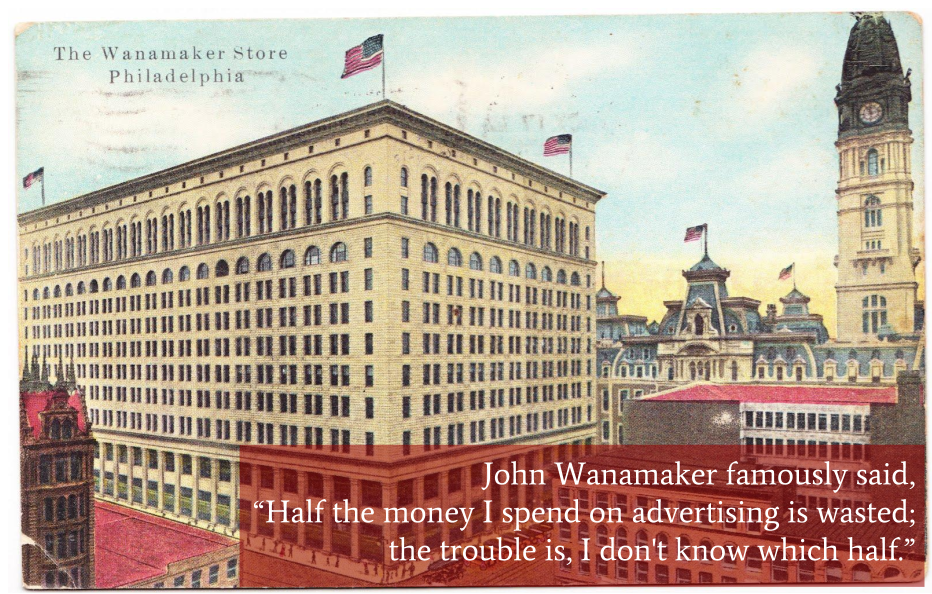
\includegraphics[height=\textheight]{images/WanamakerQuote.png}
\source{\href{http://www.papergreat.com/2012/09/saturdays-postcard-wanamakers-and-1911.html}{Papergreat blog}}
\end{frame}

\begin{frame}{Measuring advertising response}
The goal of any marketing campaign is to increase sales (short-term or long-term). \\
\bigskip \pause
In theory, it should be easy to evaluate the performance of marketing.  Each campaign or marketing channel should be evaluated based on the \alert{incremental profit} that it produces relative to its \alert{cost}. \\
\bigskip
\begin{equation*}
ROI = \frac{\textnormal{incremental profit due to advertising} - \textnormal{cost of advertising}}{\textnormal{cost of advertising}}
\end{equation*}
\end{frame}

\begin{frame}{Incremental sales}
\begin{columns}[T]
\column{0.4\textwidth}
Incremental profit depends on \alert{incremental sales} which are the additional sales we make with advertising over an above what we would have sold without advertising. Incremental profit is typically a function of the incremental sales.\\
\bigskip 
\onslide<2->{With today's digital media -- where we can track individual users -- it is now possible to estimate incremental sales in many situations.}\\
\column{0.6\textwidth}
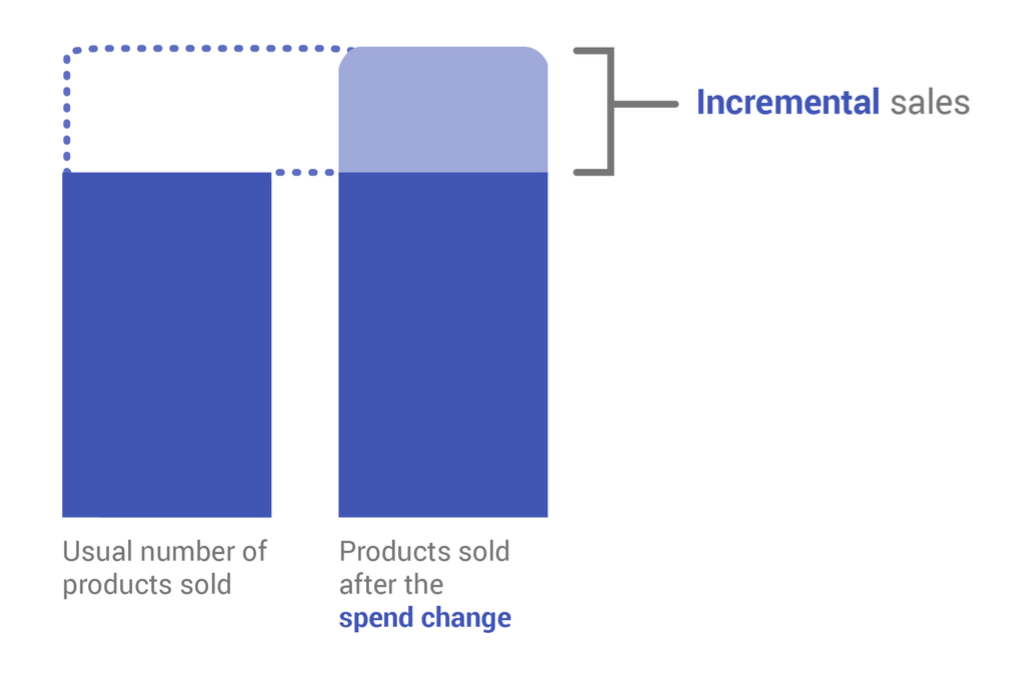
\includegraphics[width=\textwidth]{images/incremental_sales.png}
\end{columns}
\source{\href{https://www.thinkwithgoogle.com/articles/proving-marketing-impact.html}{Think with Google}}
\end{frame}

\begin{frame}{Workshop goals}
Understand four popular techniques for estimating the incremental sales due to advertising. \\
\begin{itemize}
\item Attribution rules
\item Holdout testing
\item Marketing mix modeling (with aggregate spending and sales data)
\item Attribution modeling (with user-level data)
\end{itemize}
\bigskip \pause
Learn how each technique works using the R statistical language. \\
\bigskip \pause
Understand which techniques produce better estimates of incremental profits and why.\\
\bigskip \pause
\alert{After this workshop, you won't be an expert, but you will have a much better idea of how these techniques work and you will be a much better consumer of attribution analysis that is done for you.}
\end{frame}

\begin{frame}{What if I don't know R?}
I will assume that you have some familiarity with regression, but I don't expect everyone here knows R.\\
\bigskip \pause
There are two ways to follow this tutorial: 
\begin{enumerate}
\pause 
\pause 
\item \alert{``Go for a ride"}
\begin{itemize}
\item Focus on the data that goes into the analysis and the output of the analysis, and how we interpret it. 
\item Don't worry too much about the R syntax. Let me ``drive" that. 
\item Review the R code later to learn the syntax (if you want).
\end{itemize}
\pause \item \alert{``Practice driving"}
\begin{itemize}
\item For those comfortable using R and to do data manipulation and regression (all base R, no tidyverse), download the code file and follow along. 
\end{itemize}
\end{enumerate}
\bigskip \pause
I don't intend to teach you R.  I'm just using because it is my favorite platform for data manipulation, computing summary statistics, graphing and regression modeling. This analysis could be done using Python/Pandas, SAS, Matlab, etc.
\end{frame}

\subsection{Data}

\begin{frame}{Data: retail impressions and conversions}
Throughout this workshop, we will be analyzing a data set describing 10,000 customers and potential customers of a retailer. The retailer uses four different advertising channels. 
\begin{columns}[T]
\column{0.25\textwidth}
\centering
\textcolor{red}{Display}

\includegraphics[width=\textwidth]{images/target_display.png} 
\column{0.25\textwidth}
\centering
\textcolor{red}{Social}

\includegraphics[width=\textwidth]{images/target_social.png}
\column{0.25\textwidth}
\centering
\textcolor{red}{Email}
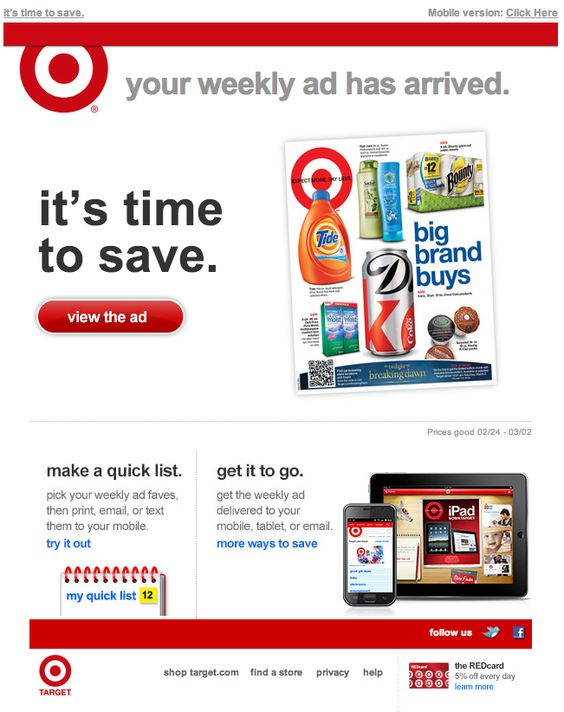
\includegraphics[width=\textwidth]{images/target_email.jpg}
\column{0.25\textwidth}
\centering
\textcolor{red}{Direct}

\includegraphics[width=\textwidth]{images/target_direct.jpeg}
\end{columns}
Customer tracking begins when the customer is exposed to a display or social ad, visits the retailer website or makes a purchase. 
\end{frame}

\begin{frame}{Data structure}
The data is organized in three files: \\
\begin{itemize}
\item \texttt{customer.csv}: \textcolor{gray}{each row is a customer, 10,000 rows}
\item \texttt{impressions.csv}: \textcolor{gray}{each row is an exposure of a marketing communication to a specific customer, 501,336 rows}
\item \texttt{transactions.csv}: \textcolor{gray}{each row is a transaction made by a customer}
\end{itemize}
\pause This basic structure is typical of raw digital advertising data. The data is hypothetical -- I made it in R -- and has been designed to illustrate important points in data analysis. \\
\end{frame}

\begin{frame}[fragile]{Some R preliminaries}
We start our R session with a bit of tidying up. 
\begin{lstlisting}
> rm(list=ls()) # clears the workspace
> set.seed("20030603") # ensures repeatable results for attribution rules
> options(scipen=999) # suppress scientific notation
\end{lstlisting}
\end{frame}

\subsubsection{Customer file}

\begin{frame}[fragile]{\alert{Customer file}}
The customer file can be downloaded from \href{https://goo.gl/mqy8NR}{https://goo.gl/mqy8NR}. Each row describes a customer. \\
\bigskip
\emph{Columns:} \\
\verb|id|: \textcolor{gray}{an id number for the customer}\\
\verb|past purchase|: \textcolor{gray}{whether the customer has made a purchase prior to the observation period.} \\
\verb|email|: \textcolor{gray}{indicates whether the customer is eligible to receive emails, i.e. we have an email address and permission to mail}\\
\verb|direct|: \textcolor{gray}{indicates whether the customer is eligible to receive direct mail, i.e. we have an address and permission to mail}\\
\end{frame}

\begin{frame}[fragile]{Read and inspect \alert{customer file}}
We can read the file directly into R: 
\begin{lstlisting}
> cust <- read.csv("https://goo.gl/mqy8NR")
> nrow(cust)
[1] 10000
> summary(cust)
       id        past.purchase        email            direct      
 Min.   :    1   Min.   :0.0000   Min.   :0.0000   Min.   :0.0000  
 1st Qu.: 2501   1st Qu.:0.0000   1st Qu.:0.0000   1st Qu.:0.0000  
 Median : 5000   Median :1.0000   Median :1.0000   Median :0.0000  
 Mean   : 5000   Mean   :0.5022   Mean   :0.6001   Mean   :0.4974  
 3rd Qu.: 7500   3rd Qu.:1.0000   3rd Qu.:1.0000   3rd Qu.:1.0000  
 Max.   :10000   Max.   :1.0000   Max.   :1.0000   Max.   :1.0000  
\end{lstlisting}
\alert{We have 10,000 customers and about half of those have made a purchase. About 60\% are eligible for email and 50\% are eligible for direct mail.}
\end{frame}

\begin{frame}[fragile]{More inspection of \alert{customer file}}
\begin{lstlisting}
> xtabs(~email+direct+past.purchase, data=cust)
, , past.purchase = 0
     direct
email    0    1
    0 2775  707
    1 1205  291
, , past.purchase = 1
     direct
email    0    1
    0   95  422
    1  951 3554
\end{lstlisting}
\alert{Most customers who have not made a purchase are not eligible for email or direct mail. Customers who have made a purchase are more likely to be eligible.}
\end{frame}

\subsubsection{Impressions file}

\begin{frame}[fragile]{\alert{Impressions file}}
The impressions file can be downloaded from \href{https://goo.gl/74qIxy}{https://goo.gl/74qIxy}. Each row in the file represents an exposure of one customer to an ad, i.e. an impression.\\
\bigskip
\emph{Columns:} \\
\verb|id|: \textcolor{gray}{id number for the customer}\\
\verb|date|: \textcolor{gray}{date of impression. Most files would have a date-time, but we have simplified for the workshop.}  \\
\verb|channel|: \textcolor{gray}{channel of the ad exposure} \\
\verb|click|: \textcolor{gray}{indicates whether the customer clicked on the ad} \\
\end{frame}

\begin{frame}[fragile]{Read and inspect \alert{impressions file}}
\begin{lstlisting}
> impress <- read.csv("https://goo.gl/74qIxy")
> impress$date <- as.Date(impress$date) # change type
> nrow(impress)
[1] 501336
> summary(impress)
       id             date                     channel           click        
 Min.   :    1   Min.   :2016-12-31   direct       :  9948   Min.   :0.00000  
 1st Qu.: 2467   1st Qu.:2017-01-10   display      :216371   1st Qu.:0.00000  
 Median : 4940   Median :2017-01-20   email        : 38426   Median :0.00000  
 Mean   : 4960   Mean   :2017-01-22   email.holdout:  9582   Mean   :0.01854  
 3rd Qu.: 7454   3rd Qu.:2017-01-31   social       :227009   3rd Qu.:0.00000  
 Max.   :10000   Max.   :2017-02-27                          Max.   :1.00000  
\end{lstlisting}
\alert{We have 501,336 impressions between 2016-12-31 to 2017-02-27.  The majority of these impressions are social or display.  Overall click rate is 1.85\%, which is reasonable.}
\end{frame}

\begin{frame}[fragile]{Summarize the cadence of the impressions}
\alert{Cadence} is the timing of advertising impressions.  It is useful to understand the cadence of your ads before you do any other analysis. Email and direct are often sent out to users on specific dates.  Display and social ads can be steady or can be turned on and off at specific times. We can summarize the cadence with the crosstab function in R.
\begin{lstlisting}
> (cadence <- xtabs(~date+channel, data=impress))  
            channel
date         direct display email email.holdout social
  2016-12-31      0     788     0             0   1610
  2017-01-01      0    3786     0             0   7481
  2017-01-02      0    3792     0             0   7416
  2017-01-03      0    3656  4798          1203   7505
  2017-01-04      0    3731     0             0   7648
  ...
\end{lstlisting}
\end{frame}

\begin{frame}[fragile]{Visualizing the cadence}
It is useful to create plot of the cadence data. 
\begin{lstlisting}
> cadence <- cadence[,c(2,5,1,3,4)] # reorder the columns
> mycols <- c("gray50", "wheat2", "darkorange2", "steelblue2", "steelblue4")
> barplot(t(cadence), col=mycols, ylab="impressions") 
> legend("topright", legend=colnames(cadence), fill=mycols, cex=0.6)
\end{lstlisting}
\end{frame}

\begin{frame}{Visualizing the cadence}
\begin{center}
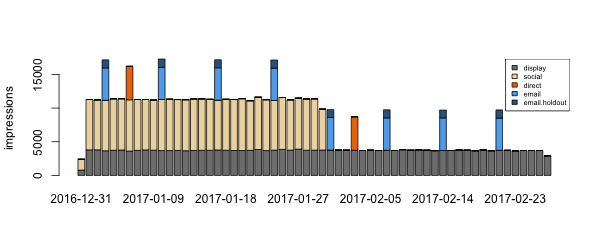
\includegraphics[width=.85\textwidth]{images/cadence.png}
\end{center}
\alert{Display impressions per day are steady across the observation window. \\
Social is steady in the first month and then stops. \\
Emails are sent once per week and each campaign seems to have a holdout.  \\
Direct mail is sent once per month.}
\end{frame}

\begin{frame}[fragile]{Histogram of impressions}
It is also useful to understand how many impressions each customer gets. 
\begin{lstlisting}
> hist(xtabs(~id, data=impress), xlab="Impressions", ylab="Count of Users",
+      main="Histogram of Impressions per User")
\end{lstlisting}
\begin{center}
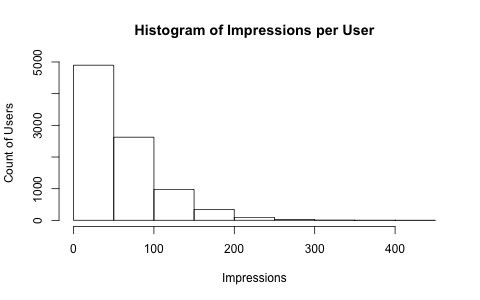
\includegraphics[height=.5\textheight]{images/histimpressions.png}
\end{center}
\alert{Some customers receive as many as 400 impressions in two months, but most get less than 100 impressions.}
\end{frame}

\begin{frame}[fragile]{Click through rates by channel}
\begin{lstlisting}
> xtabs(click~channel, data=impress)/xtabs(~channel, data=impress)
channel
       direct       display         email email.holdout        social 
  0.000000000   0.004783451   0.099672097   0.000000000   0.019519050 
\end{lstlisting}
\alert{The click through rates are highest for email at 10.0\% and lowest for display at 0.5\%.  As expected, there are no clicks for direct or email holdouts.}
\end{frame}

\subsubsection{Transactions file}

\begin{frame}[fragile]{\alert{Transactions file}}
The transactions file can be downloaded from \href{https://goo.gl/lIAuZu}{\texttt{https://goo.gl/lIAuZu}}. Each row in the file represents a purchase made by a customer. \\
\bigskip
Columns: \\
\verb|id|: id number for the customer \\
\verb|date|: date of transactions. Most files would have a date-time, but we have simplified for the workshop.  \\
\verb|last.touch|: channel of the last ad impression the customer saw before the transaction\\
\verb|last.click|: channel of the last ad the customer clicked before the transaction\\
\bigskip
Purchase amounts can be used in holdout testing, attribution models or marketing mix models, but we will focus on transaction counts for this workshop.\\
\end{frame}

\begin{frame}[fragile]{Read and inspect \alert{transactions file}}
\begin{lstlisting}
> summary(trans)
       X               id             date              last.touch     last.click   
 Min.   :    1   Min.   :    2   Min.   :2017-01-01   direct :2594   display:  891  
 1st Qu.: 5609   1st Qu.: 2472   1st Qu.:2017-01-12   display:5252   email  : 4151  
 Median :11217   Median : 5005   Median :2017-01-25   email  :7145   none   :12998  
 Mean   :11217   Mean   : 4985   Mean   :2017-01-26   none   : 846   social : 4393  
 3rd Qu.:16825   3rd Qu.: 7483   3rd Qu.:2017-02-08   social :6596                  
 Max.   :22433   Max.   :10000   Max.   :2017-02-28  
\end{lstlisting}
\alert{The transactions span the same dates and customer ids as the impressions.  It looks like some customers such as id 1 do not have transactions.}
\end{frame}

\begin{frame}[fragile]{Transactions over time}
\begin{lstlisting}[basicstyle=\tiny\ttfamily]
> (transbyday <- xtabs(~date, data=trans))
date
2017-01-01 2017-01-02 2017-01-03 2017-01-04 2017-01-05 2017-01-06 2017-01-07 2017-01-08 
       325        357        589        479        403        498        564        586 
2017-01-09 2017-01-10 2017-01-11 2017-01-12 2017-01-13 2017-01-14 2017-01-15 2017-01-16 
       556        660        539        422        317        315        348        356 
2017-01-17 2017-01-18 2017-01-19 2017-01-20 2017-01-21 2017-01-22 2017-01-23 2017-01-24 
       577        512        428        357        324        336        355        561 
2017-01-25 2017-01-26 2017-01-27 2017-01-28 2017-01-29 2017-01-30 2017-01-31 2017-02-01 
       475        349        334        342        327        317        507        373 
2017-02-02 2017-02-03 2017-02-04 2017-02-05 2017-02-06 2017-02-07 2017-02-08 2017-02-09 
...
\end{lstlisting}
\alert{This is easier to understand if we plot it.} 
\end{frame}

\begin{frame}[fragile]{Plot of transactions over time}
\begin{lstlisting}
> plot(transbyday, ylab="Transactions", xlab="Date")
\end{lstlisting}
\begin{center}
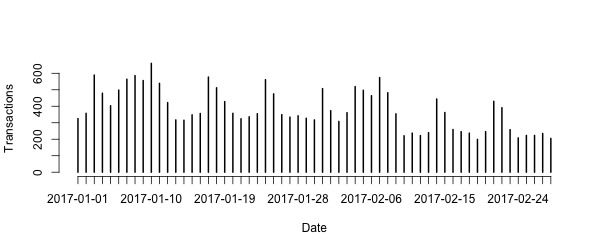
\includegraphics[height=0.6\textheight]{images/transbyday.png}\\
\end{center}
\alert{Transactions appear to be a bit higher in the first month and there are clear spikes around the time of emails and direct mail.}
\end{frame}

\begin{frame}[fragile]{Histogram of transactions}
\begin{lstlisting}
> hist(xtabs(~id, data=trans), xlab="Number of Transactions", ylab="Count of Users", 
+      main="Histogram of Transactions")
\end{lstlisting}
\begin{center}
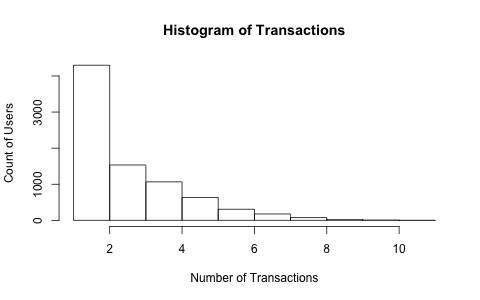
\includegraphics[height=0.5\textheight]{images/histtrans.png}
\end{center}
\alert{Most customers have less than 2 transactions in the two month observation period.}
\end{frame}

\begin{frame}[fragile]{Customer 100}
To understand how the files fit together, it is helpful to look at the impressions and transactions for one customer. 
\begin{lstlisting}
> cust[cust$id==100,]
     id past.purchase email direct
100 100             0     0      0
> impress[impress$id==100,]
[1] id      date    channel click  
<0 rows> (or 0-length row.names)
> trans[trans$id==100,]
      X  id       date last.touch last.click
206 206 100 2017-01-18       none       none
207 207 100 2017-01-26       none       none
\end{lstlisting}
\alert{Customer 100 has no impressions and made two transactions.} 
\end{frame}

\begin{frame}[fragile]{Customer 300}
\footnotesize
\begin{lstlisting}
> cust[cust$id==300,]
     id past.purchase email direct
300 300             1     1      1
> summary(impress[impress$id==300,])
       id           date                     channel       click  
 Min.   :300   Min.   :2016-12-31   direct       : 2   Min.   :0  
 1st Qu.:300   1st Qu.:2017-01-10   display      :81   1st Qu.:0  
 Median :300   Median :2017-01-29   email        : 8   Median :0  
 Mean   :300   Mean   :2017-01-28   email.holdout: 0   Mean   :0  
 3rd Qu.:300   3rd Qu.:2017-02-14   social       : 0   3rd Qu.:0  
 Max.   :300   Max.   :2017-02-26                      Max.   :0  
> trans[trans$id==300,]
      X  id       date last.touch last.click
647 647 300 2017-01-03    display       none
648 648 300 2017-01-10      email       none
649 649 300 2017-02-04     direct       none
650 650 300 2017-02-19    display       none
\end{lstlisting}
\alert{Customer 300 has 8 email, 2 direct mail and 81 display impressions and made 4 transactions.}
\end{frame}

\begin{frame}{Steps in data inspection}
\begin{enumerate}
\item For each file, 
\begin{enumerate}
\item Make sure you have the entire file read in by checking number of rows.
\item Summarize individual variables in file mean, min, max, etc.  Do they make sense?
\item Summarize relationships between variables in file using crosstabs or scatterplots.  Do they make sense?
\end{enumerate}
\item Check that joins between files are as expected (skipped).
\item Summarize relationships between files.  Do they make sense? 
\end{enumerate}
\end{frame}

\section{Attribution rules}

\subsection{What is last click?}

\begin{frame}{Last-touch attribution}
\alert{Last-click} (or \alert{last-touch}) attribution looks backward from each conversion to find the last ad the user clicked on prior to the conversion.\\
\bigskip
\centering
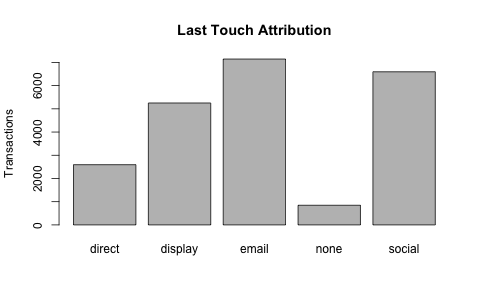
\includegraphics[height=0.5\textwidth]{images/lasttouch.png}\\
\source{\href{http://www.digitaldealer.com/marketing-attribution-finally-connects-dots/}{Digital Dealer}}
\bigskip \pause
\alert{This is (obviously?) a bad idea.}
\end{frame}
 
\subsection{Last touch analysis in R}

\begin{frame}[fragile]{Last touch analysis}
The last click and the last touch are stored in the transaction file.
\begin{lstlisting}
> head(trans)
  id       date last.touch last.click
1  2 2017-01-04      email       none
2  2 2017-02-12      email       none
3  3 2017-02-02      email       none
4  3 2017-02-14      email       none
5  5 2017-01-04    display      email
6  5 2017-01-13    display      email
\end{lstlisting}
One advantage of last-click is that it is easy to compute once this pre-processing is done. 
\end{frame}

\begin{frame}[fragile]{Last touch analysis}
For example, if we want to compute the number of transactions that are attributed to each channel by last touch, we just do a quick crosstab on the transaction table.   
\begin{lstlisting}
> (last.touch.att <- xtabs(~last.touch, data=trans))
last.touch
 direct display   email    none  social 
   2594    5252    7145     846    6596 
> barplot(last.touch.att, ylab="Transactions", 
+         main="Last Touch Attribution")
\end{lstlisting}
\alert{When we do this, we are ignoring all the customers who didn't transact.}
\end{frame}

\begin{frame}[label=lasttouch]{Last touch analysis}
\begin{center}
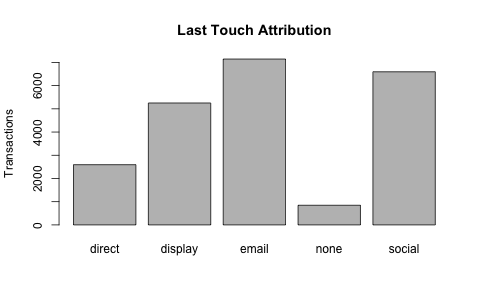
\includegraphics[width=0.5\textwidth]{images/lasttouch.png}
\end{center}
\alert{Many people interpret this as meaning that the incremental sales for social are 6596.}
\end{frame} 

\begin{frame}[fragile]{Last touch for subgroups of transactions}
It is also easy to compute the last touch for a subgroup of the transactions. Simply subset out the transactions of interest and then crosstab.
\begin{lstlisting}
> xtabs(~last.touch, data=trans[trans$date>as.Date("2017-01-31"),])
last.touch
 direct display   email    none  social 
   1669    2682    4081     258     328 
\end{lstlisting}
\alert{In February, there were far fewer sales attributed to social, most likely because we ended the social ads at the end of January.}
\end{frame}

\begin{frame}[fragile]{Last click analysis}
\begin{columns}
\column{0.65\textwidth}
You can do the same analysis based on the last ad a customer clicked, rather than the last touch/impression. 
\footnotesize
\begin{lstlisting}
> (last.click.att <- xtabs(~last.click, data=trans))
last.click
display   email    none  social 
    891    4151   12998    4393 
> barplot(last.click.att, ylab="Transactions", 
+         main="Last Click Attribution")
\end{lstlisting}
\column{0.35\textwidth}
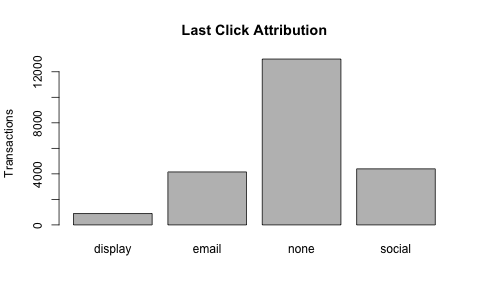
\includegraphics[width=\textwidth]{images/lastclick.png}
\end{columns}
\alert{Since people don't click very much, the attributed sales are much lower. Measuring ad performance based on clicks doesn't make much sense for the advertiser.}
\end{frame}

\begin{frame}[fragile]{Appending last click data [bonus R material]}
This function takes a transaction table that does not include the last touch and appends it based on the impression table. 
\footnotesize
\begin{lstlisting}[basicstyle=\tiny\ttfamily]
append.last <- function(trans, impress) {
  out <- data.frame(trans, last.touch=NA, last.click=NA)
  for (t in 1:nrow(out)) {
    impr <- impress[impress$id==out$id[t] & impress$date<=out$date[t] &     impress$channel!="email.holdout", ]
    if (nrow(impr)>0) {
      out$last.touch[t] <- as.character(sample(impr$channel[impr$date==max(impr$date)], 1)) # choose randomly
    }
    impr <- impr[impr$click==1,]
    if (nrow(impr)>0){
      out$last.click[t] <- as.character(sample(impr$channel[impr$date==max(impr$date)], 1))
    }
  }
  out[is.na(out)] <- "none"
  out
}
trans <- append.last(trans, impress)
\end{lstlisting}
\end{frame}

\subsection{Limitations of last-click} 

\againframe{lasttouch}

\begin{frame}{Incorrect assumptions behind last touch} 
When we use last touch to estimate the incremental sales for an ad, we are making two mistakes: 
\begin{enumerate}
\item Other ads may have influenced the customer and contributed to the sale.
\begin{itemize} 
\pause \item This is the problem everyone seems to recognize.
\end{itemize}
\pause \item It counts all the sales as incremental, i.e. it assumes that customers who saw ads would not have bought if they hadn't seen the ads.
\begin{itemize}
\pause \item This issue is less well recognized.
\end{itemize}
\end{enumerate}
\end{frame}

\begin{frame}{Attribution as a payment mechanism}
Because last-touch is so simple to compute, it has been used as a rule for allocating payments between channels on pay-for-conversion ads. \\
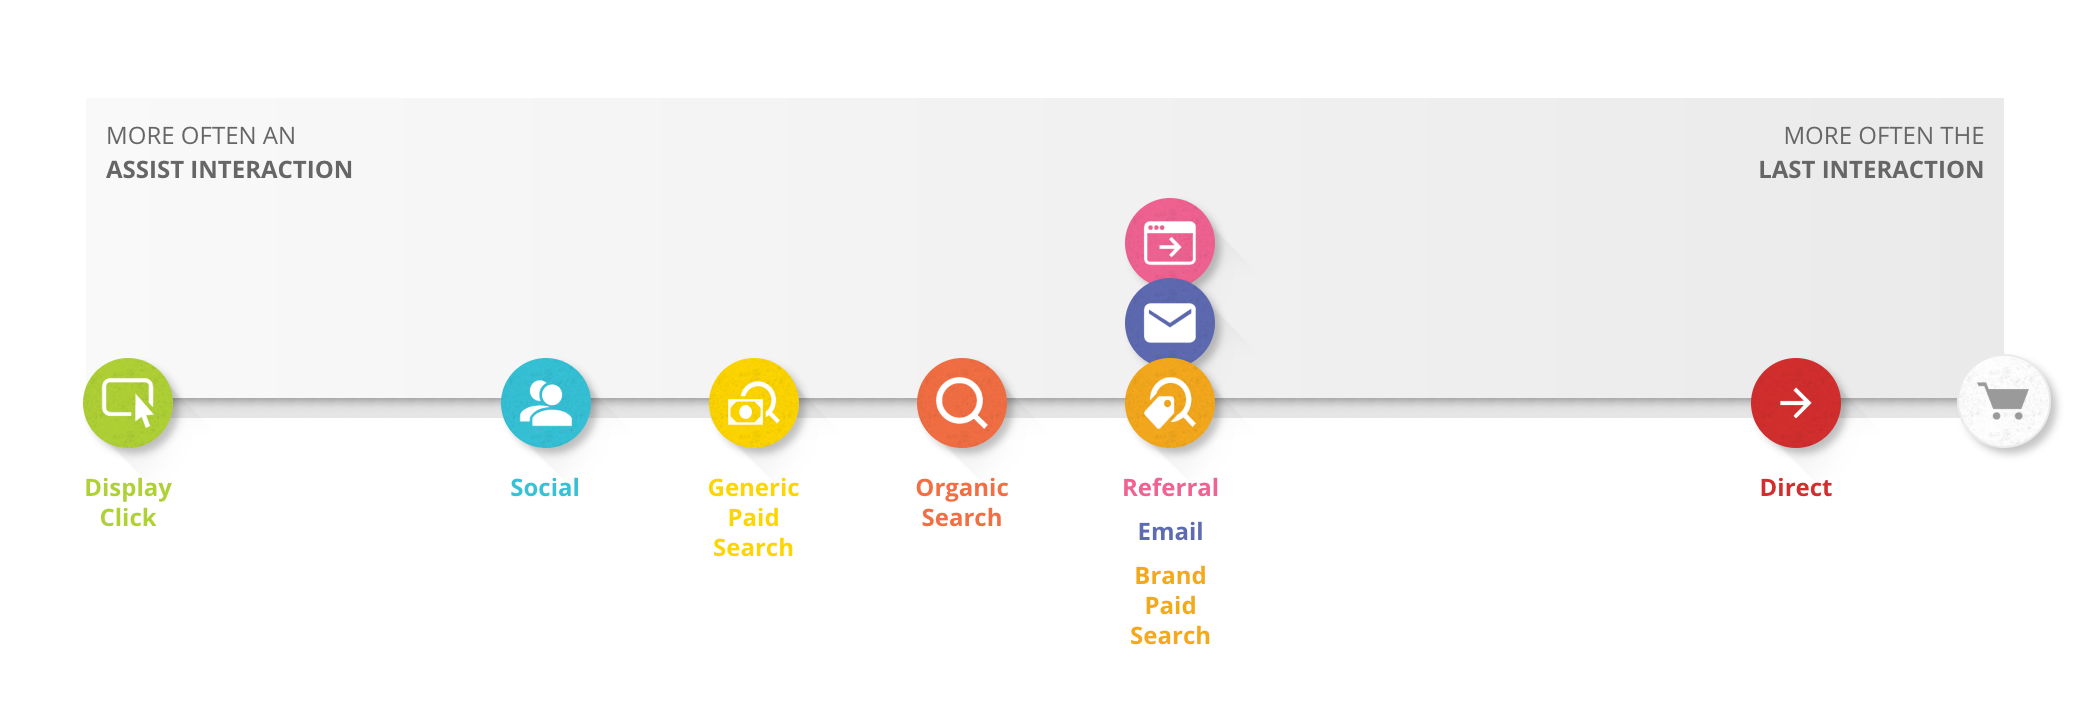
\includegraphics[width=0.8\textwidth]{images/pathtopurchase.png}
\source{\href{https://goo.gl/W3p5Tv}{Think with Google}}
\alert{Last touch unfairly favors channels that tend to show ads towards the end of the path to purchase such as search and retargeting.}
\end{frame}

\begin{frame}{Other attribution rules (``models")}
Perhaps because everyone intuitively understood that last touch didn't account for ``assists" and was unfair to channels that tend to occur early in the path to purchase they came up with other arbitrary rules. \\
\begin{center}
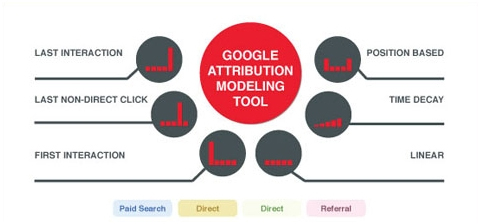
\includegraphics[height=0.4\textheight]{images/google-attribution-modeling-tool.jpg} 
\end{center}
\source{\href{http://www.a-cross.com/health/node/516}{Across Health}}
\pause
\alert{These improved rules may help problem 1, but they don't help with problem 2.}  \\
\end{frame}

\begin{frame}{When does last-touch ``work"}
Last click provides an accurate measure of ad response when
\begin{itemize}
\item All sales from customers who were exposed to ads are \alert{incremental}. That is, none of the sales would have happened without the advertising. 
\item The duration of advertising response is relatively short and the ad exposures are well spaced out over time, so that there are not other channels providing an ``assist".
\end{itemize}
These conditions might hold for a startup or a new product, but not for too many other advertisers.
\end{frame}

\begin{frame}{}
\begin{center}

\includegraphics[height=0.7\textheight]{images/lastclickdead.png}
\end{center}
\source{\href{https://www.mazeberry.com/en/blog-why-is-last-click-dead/}{Mazeberry blog}}
\end{frame}

\begin{frame}{Last touch is largely dead}
There are many vendors such as Convertro, VisualIQ and MarketShare that have provided model-based attribution solutions.
\begin{center}
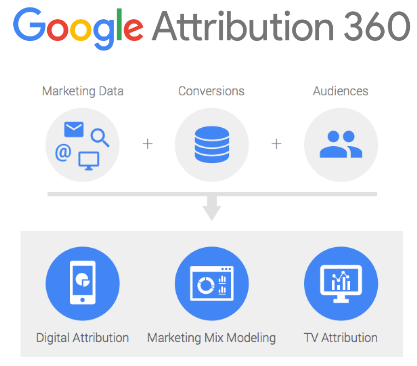
\includegraphics[height=0.5\textheight]{images/attribution360.png}
\source{\href{https://www.google.com/analytics/attribution/capabilities/}{Google Analytics 360}}
\end{center}
In Google Analytics 360, released in 2016, Google also abandoned rule-based attribution in favor of model-based approaches.
\end{frame}

\section{Holdout testing}

\subsection{What is a holdout test?}

\begin{frame}{Holdout testing}
The gold standard for measuring incremental sales is an experiment, where we \alert{randomly} assign customers to be exposed or not exposed to an ad.\\
\begin{center}
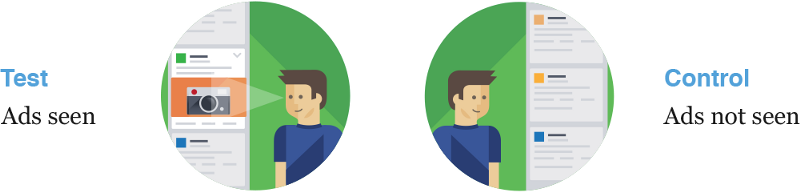
\includegraphics[width=0.8\textwidth]{images/test_control.png}
\end{center}
\source{\href{https://goo.gl/gO5Pbl}{Designing with Science, medium.com}}
For example, with email we can take our list of target emails and randomly select a set of them to not receive an email. Facebook also has a tool for randomized holdouts (for large advertisers.)
\end{frame}

\begin{frame}{Why holdout testing works}
The magic behind a holdout test is the randomization. Another name for holdout testing is \alert{randomized controlled trial}. \\
\bigskip \pause
By randomly selecting the customers for the control group, we assure that the two groups are the same on average. The treatment and control groups will be similar in their propensity to purchase and response to ads. Statisticians call this \alert{probabilistically equivalent}. 
\end{frame}

\subsection{Holdout test analysis in R}

\begin{frame}{Email holdout tests in the example data}
\begin{center}
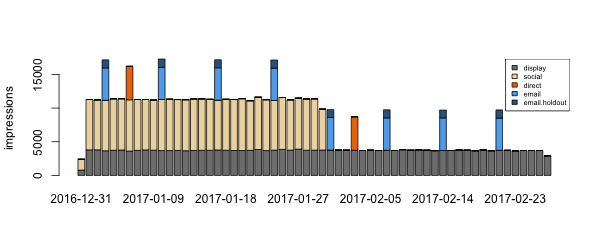
\includegraphics[width=.85\textwidth]{images/cadence.png}
\end{center}
\alert{There was an email on 2017-01-03 that included a holdout group.  Let's analyze this test.}
\end{frame}

\begin{frame}[fragile]{Function for analyzing holdout tests}
\begin{lstlisting}[basicstyle=\tiny\ttfamily]
holdout.test <- function(test.date, delay=0, window, impress, trans) {
  test.ids <- unique(impress$id[impress$channel=="email" & impress$date==test.date])
  control.ids <- unique(impress$id[impress$channel=="email.holdout" & impress$date==test.date])
  tdata <- data.frame(ids=c(test.ids, control.ids))
  tdata$group[tdata$id %in% test.ids] <- "test"
  tdata$group[tdata$id %in% control.ids] <- "control"
  in.window <- trans$date>=(test.date+delay) & trans$date<(test.date+window+delay)
  tdata$convert <- tdata$id %in% trans$id[in.window]
  ttable <- xtabs(~ group + convert, data=tdata)
  mosaicplot(~ group + convert, data=tdata, 
             main=paste("Email Test on", test.date))
  proptest <- prop.test(x=ttable[,"TRUE"], n=xtabs(~group, data=tdata))
  diff.conv <- c(diff=proptest$estimate[2]-proptest$estimate[1], ci=-proptest$conf.int)
  out <- list(diff.conv, ttable, proptest)
}
\end{lstlisting}
\end{frame}

\begin{frame}[fragile]{Analysis of email holdout test}
\begin{lstlisting}[basicstyle=\scriptsize\ttfamily]
> (holdout.test(test.date=as.Date("2017-01-03"), window=7, impress=impress, 
                trans=trans))
[[2]]
         convert
group     FALSE TRUE
  control   810  393
  test     2944 1854

[[3]]

	2-sample test for equality of proportions with
	continuity correction

data:  ttable[, "TRUE"] out of xtabs(~group, data = tdata)
X-squared = 14.395, df = 1, p-value = 0.0001482
alternative hypothesis: two.sided
95 percent confidence interval:
 -0.09011755 -0.02933788
sample estimates:
   prop 1    prop 2 
0.3266833 0.3864110
\end{lstlisting}
\end{frame}

\begin{frame}{Reporting of email holdout test}
\begin{columns}
\column{0.5\textwidth}
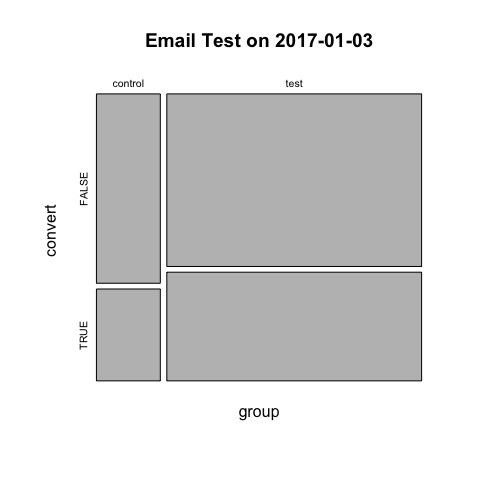
\includegraphics[width=\textwidth]{images/test1.jpeg}
\column{0.5\textwidth}
The test group had a 38.6\% conversion rate in the 7 days after the email was sent, versus a 32.7\% conversion rate for the control group. \\
\bigskip \pause
\alert{The email on 2017-01-03 produced incremental sales. The incremental increase in conversion rate is between +2.9\% and +9.0\% (95\% CI).} \\
\end{columns}
\end{frame}

\begin{frame}[fragile]{Another analysis of email holdout test on 2017-01-01}
\footnotesize
\begin{lstlisting}[basicstyle=\scriptsize\ttfamily]
 > (holdout.test(test.date=as.Date("2017-01-03"), window=3, impress=impress, trans=trans))
[[2]]
         convert
group     FALSE TRUE
  control  1063  140
  test     3850  948
  
[[3]]
	2-sample test for equality of proportions with continuity correction

data:  ttable[, "TRUE"] out of xtabs(~group, data = tdata)
X-squared = 42.187, df = 1, p-value = 0.00000000008295
alternative hypothesis: two.sided
95 percent confidence interval:
 -0.10306428 -0.05934891
sample estimates:
   prop 1    prop 2 
0.1163757 0.1975823 
\end{lstlisting}
\end{frame}

\begin{frame}{Setting the response window}
If you change the response window, you will get a different answer about how much advertising increases sales. 
\begin{itemize}
\pause \item For the email test on 2017-01-03, a response window of 3 days indicated a increase in conversion of 8.1\% (95\% CI = [5.9, 10.3]) versus 6.0\% (95\% CI = 2.9, 9.0) for a 7 day window.  
\end{itemize}
\alert{What is happening here?}
\end{frame} 

\begin{frame}{Checking ad response over time}
Ad response is often greatest just after exposure and then falls off over time.
\begin{center}
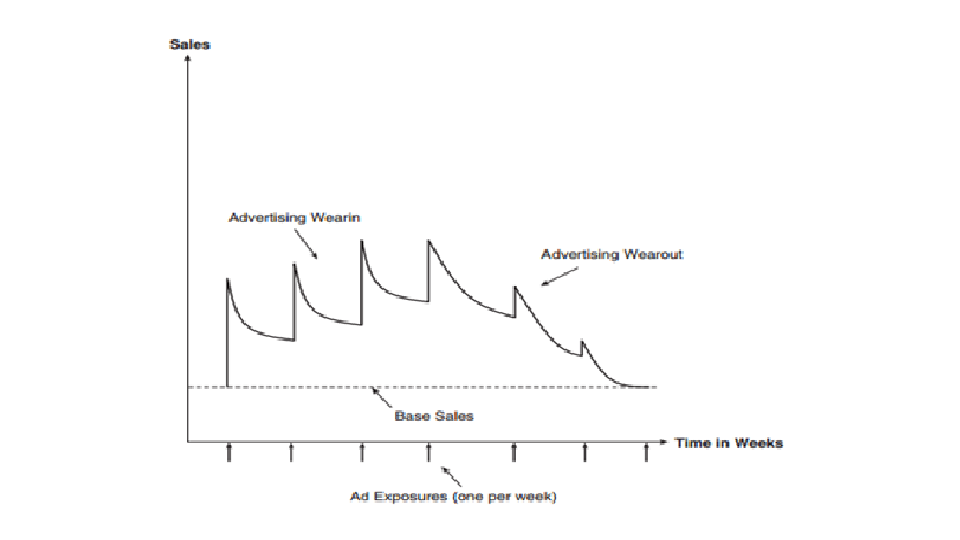
\includegraphics[height=0.7\textheight]{images/adresponseovertime.png}
\end{center}
\source{\href{https://www.linkedin.com/pulse/new-tools-determining-measuring-wear-in-wear-out-media-michael-wolfe}{Michael Wolfe}}
\end{frame}

\begin{frame}[fragile]{Ad response over time for 2017-01-03 email test}
With a holdout test, you can study the ad response over time to learn what the pattern looks like over time. \\
\begin{lstlisting}[basicstyle=\tiny\ttfamily]
day1 <- holdout.test(test.date=as.Date("2017-01-03"), delay=0, window=1, 
impress=impress, trans=trans)
...
day7 <- holdout.test(test.date=as.Date("2017-01-03"), delay=6, window=1,
impress=impress, trans=trans)
incr.conv <- c(day1[[1]][1], day2[[1]][1], day3[[1]][1], day4[[1]][1], day5[[1]][1], 
               day6[[1]][1], day7[[1]][1])
plot(incr.conv, type="h", xlab="Days after Email Sent", ylab="Increase in Conversion Rate")
abline(h=0)
\end{lstlisting}
\end{frame}

\begin{frame}{Ad response over time for 2017-01-03 email test}\
\begin{center}
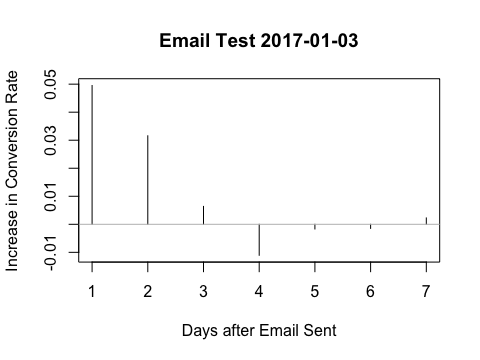
\includegraphics[height=0.7\textheight]{images/emailtestovertime.png}
\end{center}
\alert{In the test on 2017-01-03, the lift in conversion rate falls to zero in about three days.}
\end{frame}

\begin{frame}{Other email tests}
For those following along in R, try analyzing any of the other tests by modifying the code. \\
\bigskip
Dates of tests are: \\
2017-01-17 \\
 2017-01-24\\
2017-01-31 \\
 2017-02-07 \\
2017-02-14 \\
2017-02-21\\
\end{frame}

\subsection{Planning a holdout test} 

\begin{frame}{Designing a holdout test}
How do you measure response? For how long?
\begin{itemize}
\item Conversion (binary), Sales (number), or Site Visits (count)
\item During or after campaign
\end{itemize}
What advertising do the treatment and control groups receive?\\
\begin{itemize}
\item How many ads does the treatment group see? Usual? Heavy up?
\item What is used for the control? ``Go dark"? alternative ad? Usual?
\end{itemize}
Which customers are included in the test?\\
\begin{itemize}
\item Current customers, good customers or prospects? 
\end{itemize}
How should customers be assigned to treatment and control groups? \\
\begin{itemize}
\item Always random, but doesn't have to be an equal split. 
\end{itemize}
\end{frame}

\subsection{Example: Johnson, Lewis and Reiley (2017)}

\begin{frame}{Display advertising holdout test at Yahoo!}
\begin{columns}
\column{0.3\textwidth}

\includegraphics[width=\textwidth]{images/johnsonetaltest.png}\\

\includegraphics[width=\textwidth]{images/johnsonetalcontrol.png}
\source{\href{https://drive.google.com/uc?export=download&id=0B0EzanlzLNsWWDhnZ0FKOWktQ1U}{Johnson, Lewis and Reiley (2017)}}
\column{0.7\textwidth}
During two weeks in Spring 2010, a national apparel retailer ran a test on Yahoo! to measure response to \alert{display ads} on Yahoo!. \\
\bigskip
The ads displayed the retailer brand and brands of apparel firm, with slideshow transitions between photographs and text. \\
\bigskip
This test is described in detail in \href{https://drive.google.com/uc?export=download&id=0B0EzanlzLNsWWDhnZ0FKOWktQ1U}{Johnson, Lewis and Reiley (2017) ``When less is more: Data and power in advertising experiments", \textit{Marketing Science} 36(1), 43-53.}  
\end{columns}
\end{frame}

\begin{frame}{Display advertising holdout test: design}
How do you measure response? For how long?
\begin{itemize}
\item Sales (\$) at the target retailer during the two week campaign 
\end{itemize}
\pause
What advertising do the treatment and control groups receive?\\
\begin{itemize}
\item \alert{Full}: all retailer ads at all opportunities
\item \alert{Control}: house Yahoo! ads at all opportunities
\item \alert{Half}: half retailer and half house ads
\end{itemize}
\pause
Which customers are included in the test?\\
\begin{itemize}
\item Registered Yahoo! users who were also customers of the retailer were assigned to groups at the start of the two week period. Many of these users never visit Yahoo! during the campaign and don't have the opportunity to see the ads. 
\item Database match allows us to track users between Yahoo! and the retailer.
\end{itemize}
\pause
How should customers be assigned to treatment and control groups? \\
\begin{itemize}
\item Randomly, with one third in each group
\end{itemize}
\end{frame}

\begin{frame}{Display advertising holdout test: randomization checks}
It is a good idea to check that the treatment and control groups looked similar prior to the test. \\
\begin{center}
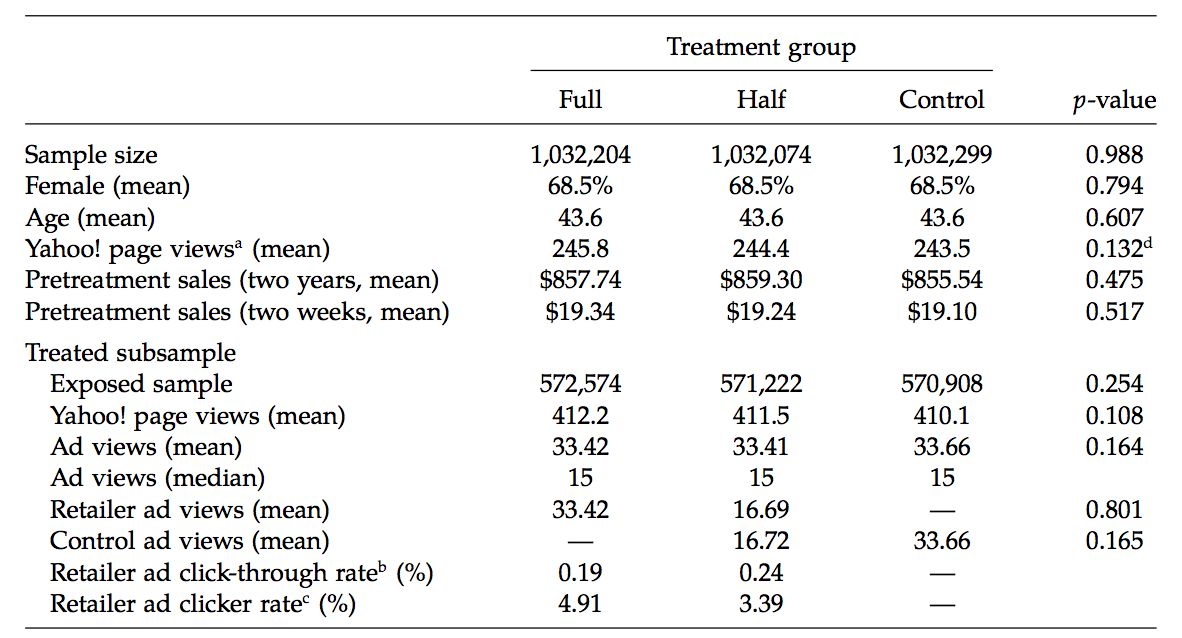
\includegraphics[height=0.4\textheight]{images/johnsonetalrandomizationcheck.png} \vspace{1cm}
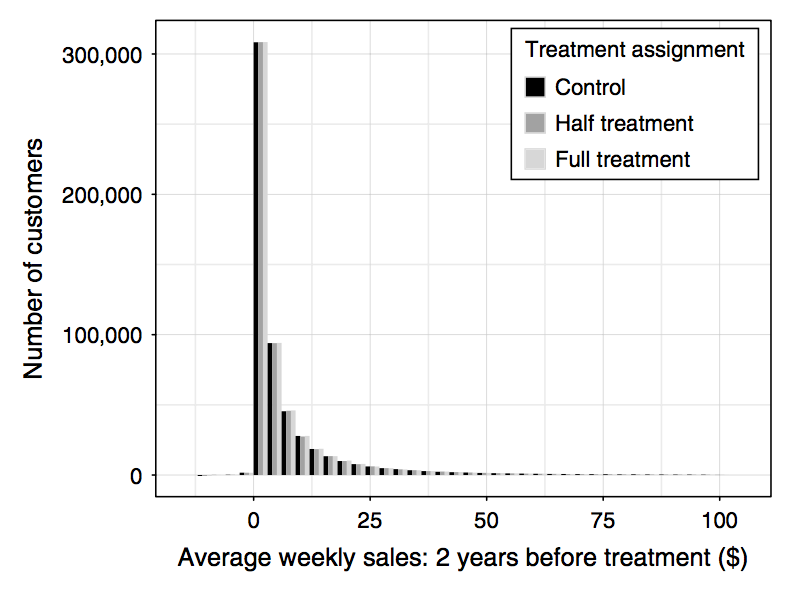
\includegraphics[height=0.4\textheight]{images/johnsonetalrandomizationcheck2.png}
\end{center}
\source{\href{https://drive.google.com/uc?export=download&id=0B0EzanlzLNsWWDhnZ0FKOWktQ1U}{Johnson, Lewis and Reiley (2017)}}
\alert{The three groups appear to be similar.  So, the randomization worked and we are comparing ``apples to apples".}
\end{frame}

\begin{frame}{Display advertising holdout test: result}
Sales Increase for Full and Half Treatments (\$)
\begin{center}
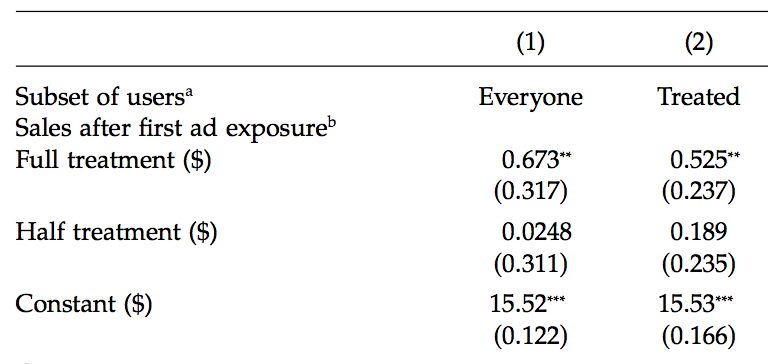
\includegraphics[height=0.5\textheight]{images/johnsonetalresult.png}
\end{center}
\alert{Looking at all the customers, the treatment increased sales by \$0.67 (95\% CI = [0.05, 1.29]). Among those who actually were exposed to ads, the effect was \$0.52 (95\% CI = [0.06,0.97]).}
\end{frame}

\subsection{Example: Gordon, Zettelmeyer, Bahargava and Chapsky (2016WP)}

\begin{frame}{Social advertising holdout test}
During two weeks in the first half of 2015, an omni-channel retailer conducted a test to determine the lift Facebook ads in the newsfeed. 
\begin{center}
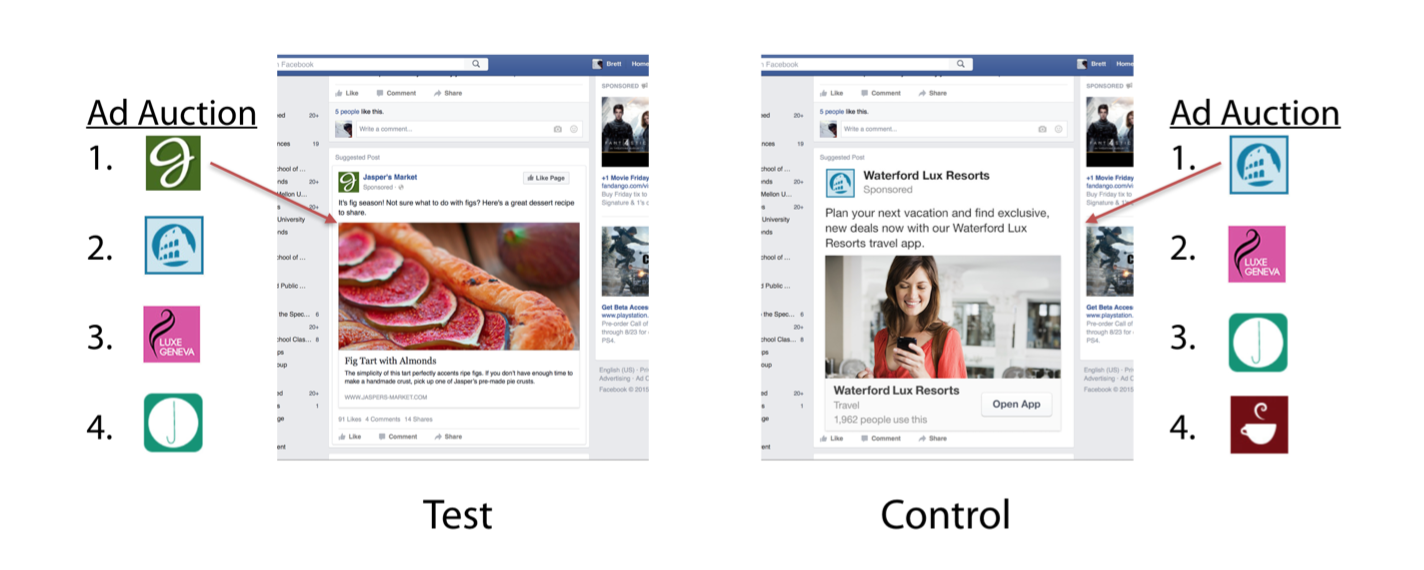
\includegraphics[height=0.5\textheight]{images/gordonetaltreatmentcontrol2.png}\\
\source{\href{https://drive.google.com/uc?export=download&id=0B0EzanlzLNsWU1BkWnFxZlZuZUE}{Gordon et al. (2016 WP)}}
\end{center}
This test is reported in \href{https://drive.google.com/uc?export=download&id=0B0EzanlzLNsWU1BkWnFxZlZuZUE}{Gordon, Zettelmeyer, Bhargava and Chapsky (2016WP) ``A Comparison of Approaches to Advertising Measurement: Evidence from Big Field Experiments at Facebook"}
\end{frame}

\begin{frame}{Search advertising holdout test design}
Which customers are included in the test?\\
\begin{itemize}
\item Facebook users that met the targeting criteria for the campaign
\end{itemize}
\pause 
How do you measure response? For how long?
\begin{itemize}
\item Purchases at the retailers website measured via Facebook conversion pixel during the campaign period and up to several weeks after the study ended.
\end{itemize}
\pause
How should customers be assigned to treatment and control groups? \\
\begin{itemize}
\item Randomly, 70\% test and 30\% control
\end{itemize}
\pause
What advertising do the treatment and control groups receive?\\
\begin{itemize}
\item Test: user is eligible to see ads and will if the retailer wins the Facebook auction
\item Control: competitor ads
\end{itemize}
\end{frame}

\begin{frame}{Social advertising holdout test: Control condition}
Since purchasing house ads or public service announcements (PSAs) is expensive, the Facebook experiment ran a competitor ad for the control. \\
\begin{center}
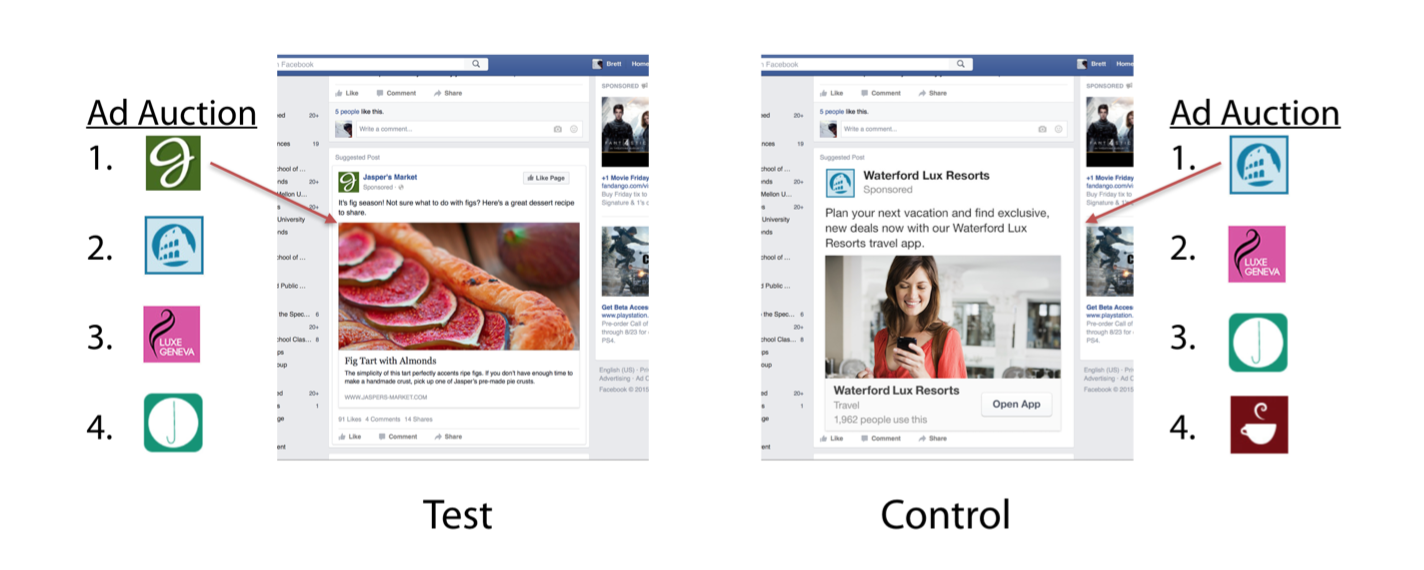
\includegraphics[height=0.5\textheight]{images/gordonetaltreatmentcontrol2.png}\\
\end{center}
\source{\href{https://drive.google.com/uc?export=download&id=0B0EzanlzLNsWU1BkWnFxZlZuZUE}{Gordon et al. (2016 WP)}}
\alert{By using the ``next advertiser" as the control condition, the sales lift we estimate is relative to ``what would have happened had we not done the campaign."}
\end{frame}


\begin{frame}{Social holdout test: Randomization check}
\begin{center}
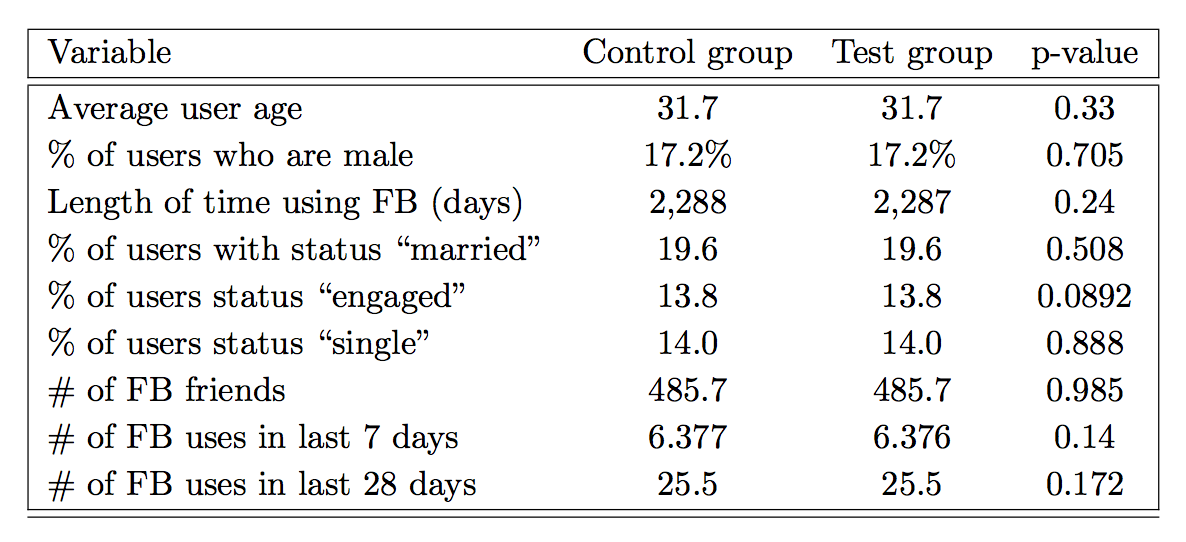
\includegraphics[height=0.6\textheight]{images/gordonetalrandomizationcheck.png}\\
\source{\href{https://drive.google.com/uc?export=download&id=0B0EzanlzLNsWU1BkWnFxZlZuZUE}{Gordon et al. (2016 WP)}}
\alert{The test and control groups appear to be similar. Randomization worked.}
\end{center}
\end{frame}

\begin{frame}{Social holdout test: Results}
\begin{center}
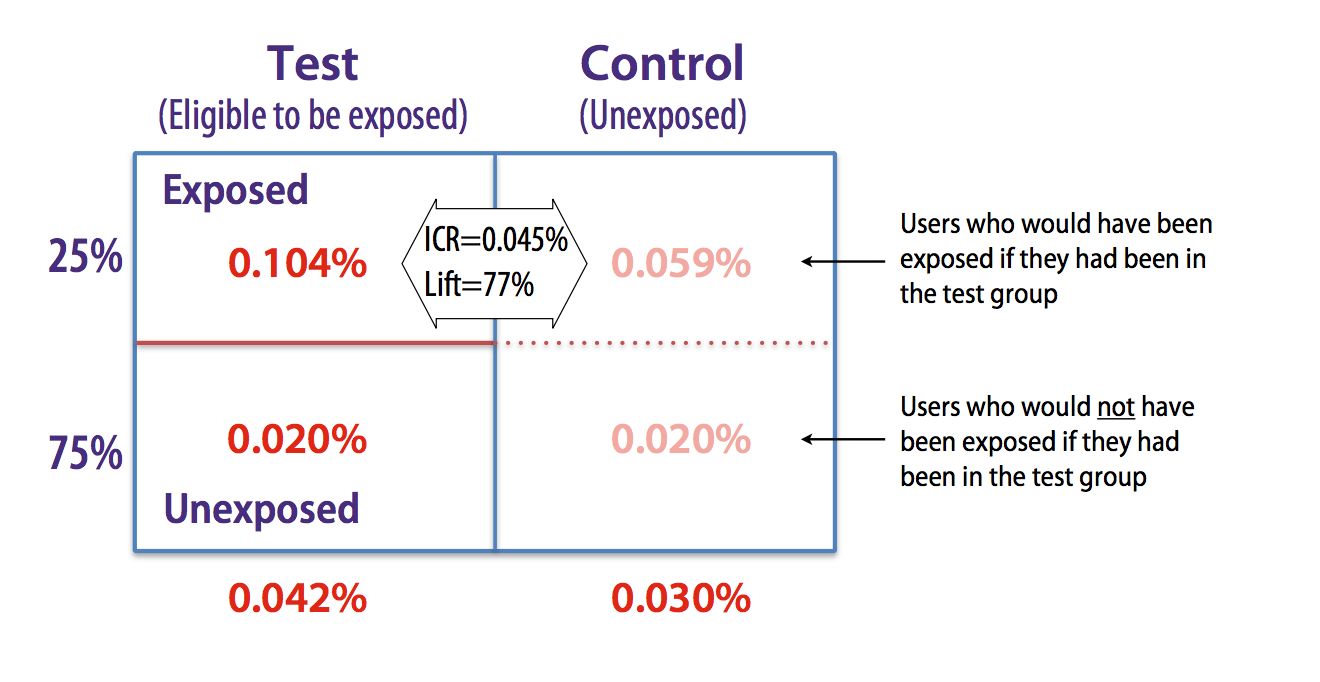
\includegraphics[height=0.6\textheight]{images/gordonetalresult.png}\\
\end{center}
\source{\href{https://drive.google.com/uc?export=download&id=0B0EzanlzLNsWU1BkWnFxZlZuZUE}{Gordon et al. (2016 WP)}}
\alert{There is a 0.045\% increase in conversions when comparing the users exposed to ads to the users in the control group that would have been exposed.}
\end{frame}

\begin{frame}{Facebook holdout testing tool: Conversion Lift}
\alert{What is conversion lift?}\\
Conversion lift accurately captures the impact that Facebook ads have in driving business for marketers. Here's how it works:
\begin{enumerate}
\item When creating a Facebook campaign, a randomized test group (people that see ads) and control group (people that don't) are established.
\item The advertiser securely shares conversion data from the campaign with Facebook. Typically, this data comes from sources like the Facebook Custom Audiences pixel, conversion pixel or secure point-of-sale (POS) data.
\item Facebook determines additional lift generated from the campaign by comparing conversions in the test and control groups.
\item The results of the study are made available in Ads Manager.
\end{enumerate}
\source{\href{https://www.facebook.com/business/news/conversion-lift-measurement}{Facebook Conversion Lift}}
\end{frame}

\begin{frame}{}
\centering
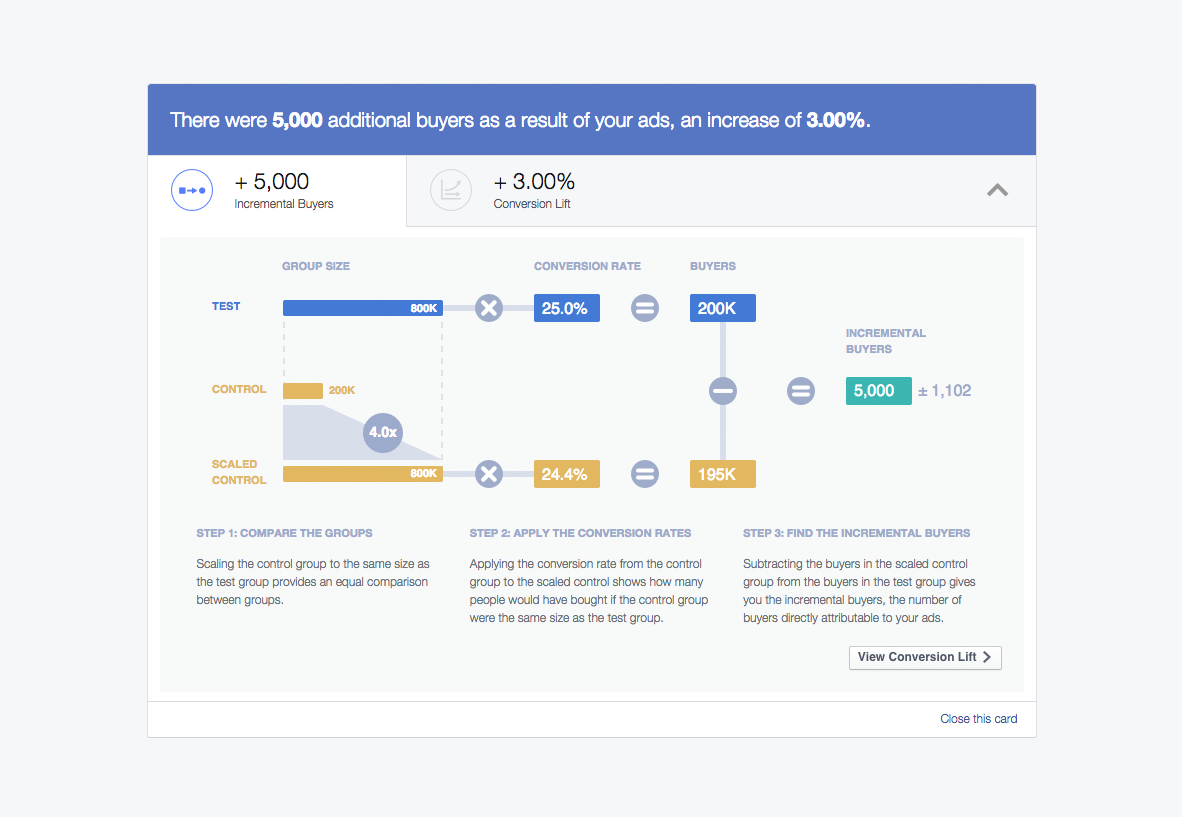
\includegraphics[height=1.2\textheight]{images/FacebookCampaignLift2.png}
\end{frame}

\subsection{Example: Blake, Nosko and Tadellis (2015)}

\begin{frame}{Search advertising holdout test}
\begin{columns}
\column{0.5\textwidth}
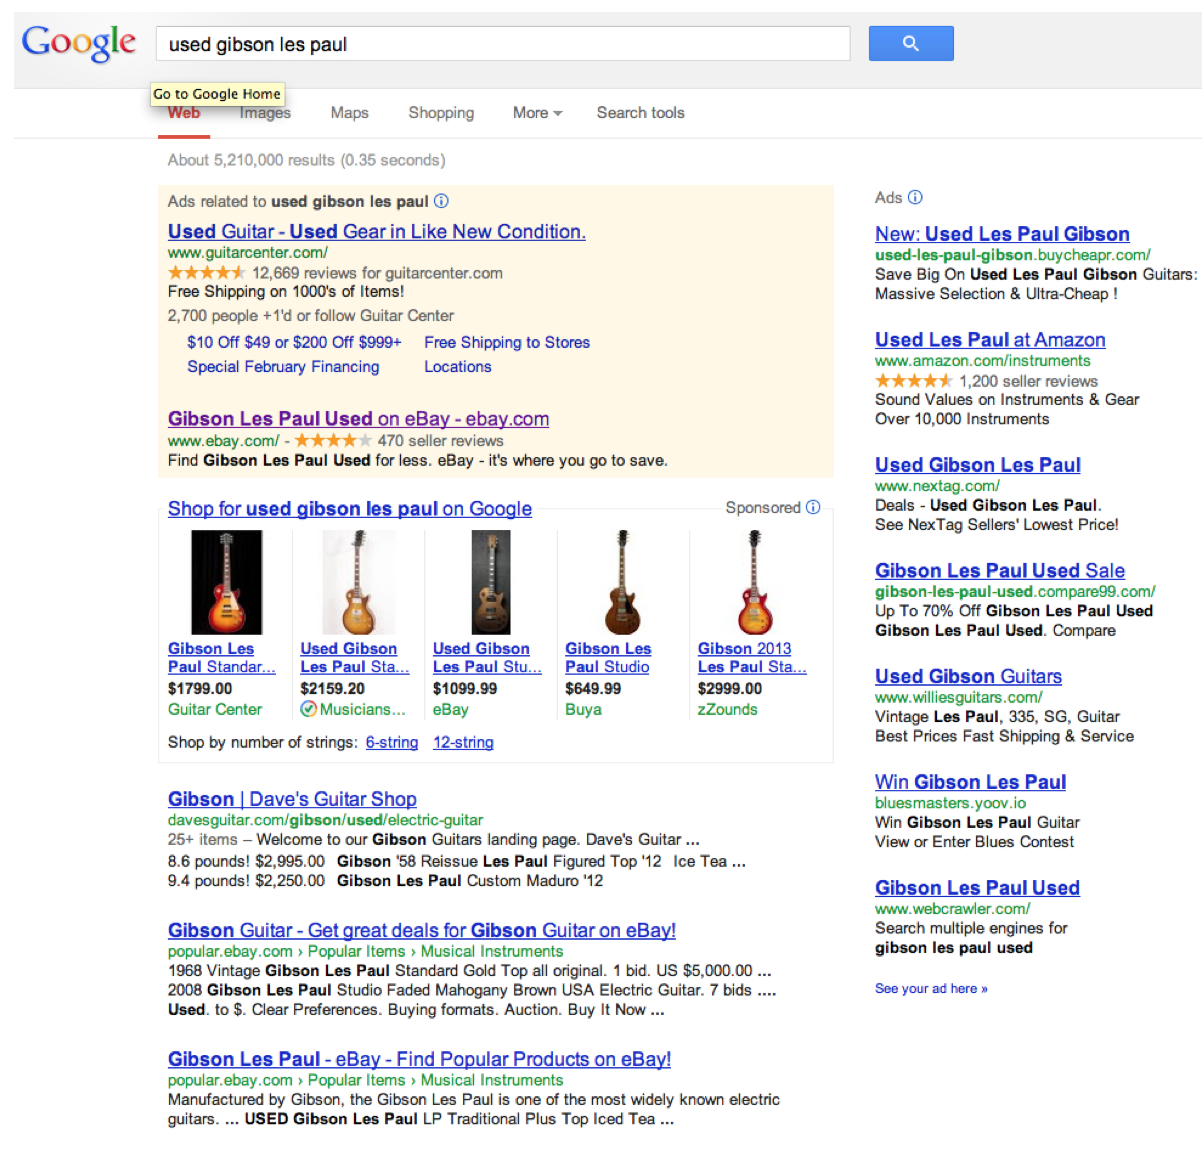
\includegraphics[height=0.8\textheight]{images/lespaul.png}
\source{\href{https://drive.google.com/uc?export=download&id=0B0EzanlzLNsWU1BkWnFxZlZuZUE}{Blake, Nosko and Tadellis (2015)}}
\column{0.5\textwidth}
In April-July 2012, eBay ran a holdout experiment to determine the sales lift of their search advertising targeting keywords other than ``eBay". \\
\bigskip
This test is reported in detail in \href{https://drive.google.com/uc?export=download&id=0B0EzanlzLNsWcUR6Y3dJVGlIazA}{Blake, Nosko and Tadelis (2015) ``Consumer Heterogeneity and Paid Search Effectiveness: A Large-Scale Field Experiment", \textit{Econometrica} 83(1), 155-174.}
\end{columns}
\end{frame}

\begin{frame}{Search advertising holdout test: Design}
Which customers are included in the test?\\
\begin{itemize}
\item Google AdWords does not provide a testing tool that will randomize search ad exposure at the user level. Instead, they conducted a \alert{geo-test} with 30\% of the DMAs in the US market. 
\end{itemize}
\pause
How do you measure response? For how long?
\begin{itemize}
\item eBay sales (\$) shipped to the DMA
\end{itemize}
\pause
What advertising do the treatment and control groups receive?\\
\begin{itemize}
\item Test: keep search advertising at usual level
\item Control: ``go dark"
\end{itemize}
\pause
How should DMAs be assigned to treatment and control groups? \\
\begin{itemize}
\item DMAs were \alert{matched} based on prior eBay sales and then randomly assigned to groups.
\end{itemize}
\end{frame}

\begin{frame}{Search advertising holdout test: Findings}
\begin{columns}
\column{0.5\textwidth}
\centering
Ratio of Sales \\ Before and During Test Period\\
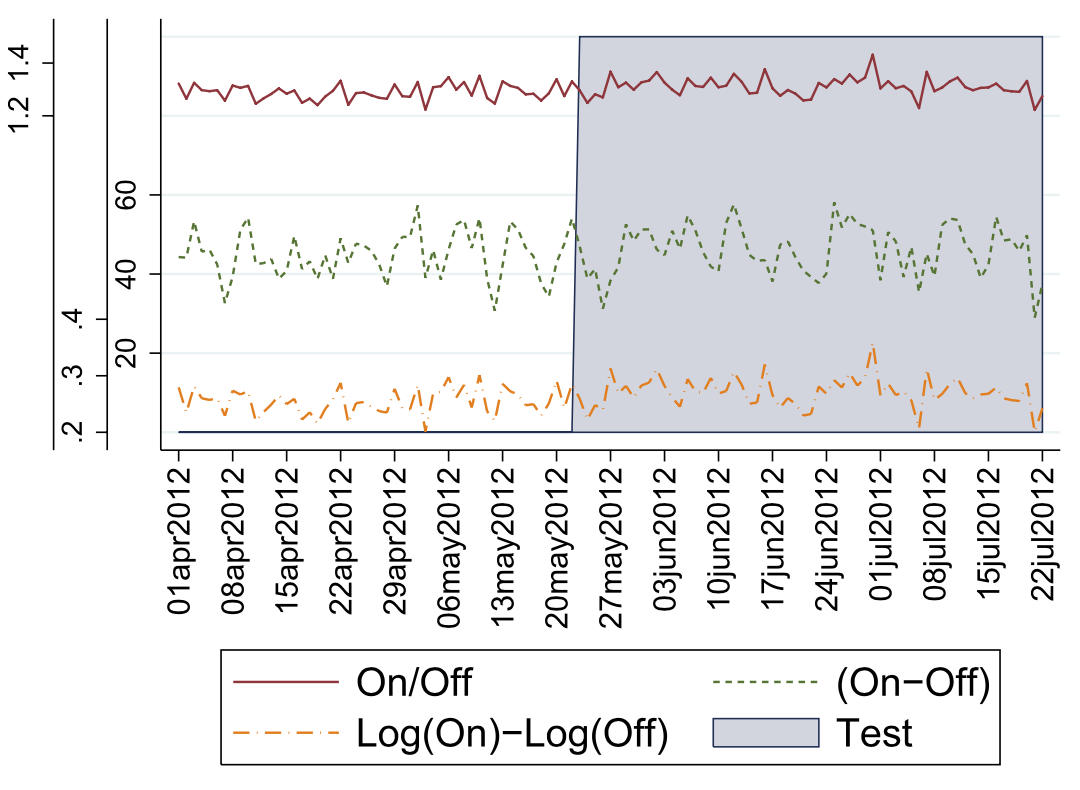
\includegraphics[width=\textwidth]{images/blakeetalresult.png}\\
\source{\href{https://drive.google.com/uc?export=download&id=0B0EzanlzLNsWU1BkWnFxZlZuZUE}{Blake, Nosko and Tadellis (2015)}}
\column{0.5\textwidth}
\alert{Search advertising does not increase eBay sales. \\ As a result, eBay has drastically reduced search advertising.}
\end{columns}
\end{frame}

\begin{frame}{Search advertising holdout test: ``Last Touch"}
\begin{columns}[t]
\column{0.5\textwidth}
\centering
``Last Touch" Attributed Sales \\
(sale within 24 hours of search ad exposure)\\
Before and During Test Period\\
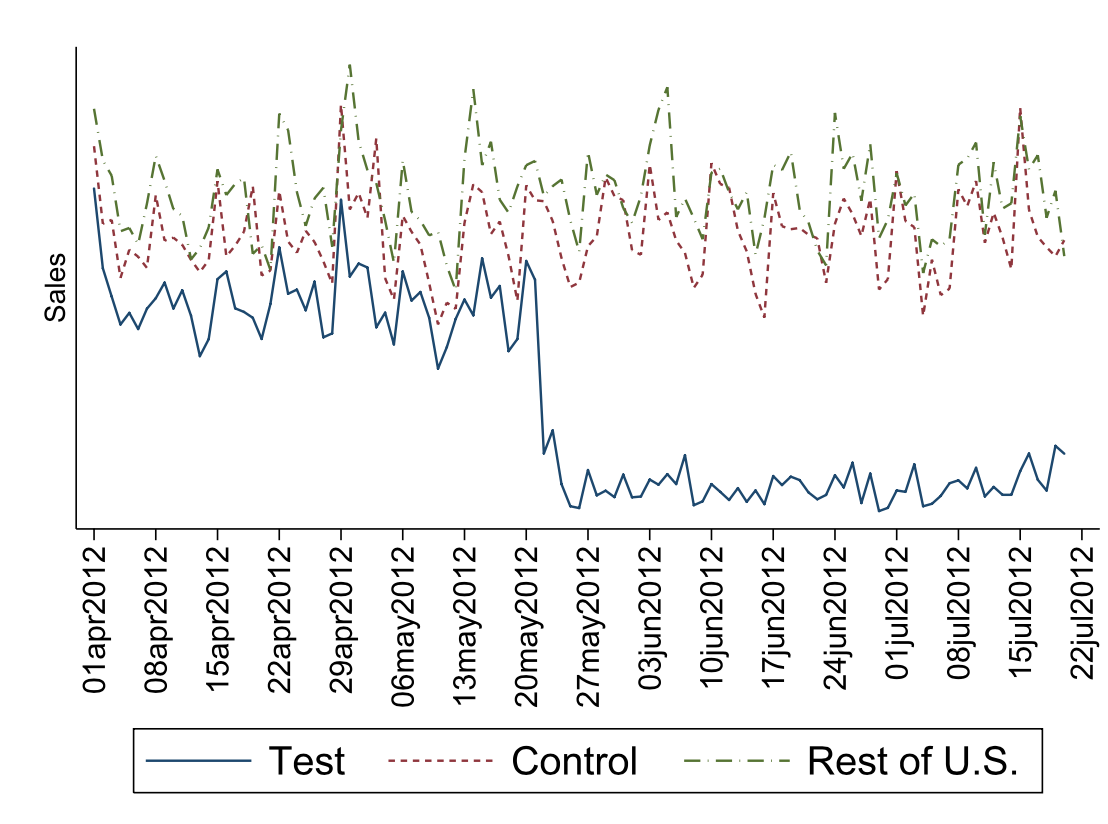
\includegraphics[width=0.9\textwidth]{images/blakeetallasttouch.png}\\
\source{\href{https://drive.google.com/uc?export=download&id=0B0EzanlzLNsWU1BkWnFxZlZuZUE}{Blake, Nosko and Tadellis (2015)}}
\column{0.5\textwidth}
\alert{If you were using last touch attribution, you would think that search advertising made a big difference.}
\end{columns}
\end{frame}

\section{Marketing mix modeling}

\subsection{What is marketing mix modeling?}

\begin{frame}{Marketing mix modeling}
Before advertisers had access to user-level ad exposure data (like our example data set) they only had data on what they had spend on advertising and (sometimes) the number of people who saw the ad. This type of spending data is similar to the aggregate impressions data we looked at for our data set. 
\begin{center}
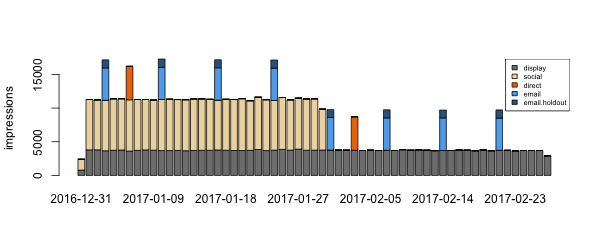
\includegraphics[width=0.6\textwidth]{images/cadence.png}
\end{center}
To find the correlation between \alert{total sales} in each day/week/month to \alert{advertising spending or impressions} on that same day/week/month, you estimate \alert{regression} model. 
\end{frame}

\begin{frame}{A simple marketing mix model}
A regression is an equation relating a response (``dependent variable") to one or more other variables (``independent variables"). \\
\bigskip \pause
A simple marketing mix model is: \\
\begin{equation*}
\textnormal{sales}_t = \alert{\beta_0} + \alert{\beta_1} \textnormal{display}_t + \alert{\beta_2}\textnormal{social}_t + \alert{\beta_3} \textnormal{email}_t + \alert{\beta_4} \textnormal{direct}_t + \epsilon_t
\end{equation*}\\
\bigskip \pause
The words represent data we have for each time period and the \alert{$\beta$}'s represent the unknown relationship between ad impressions and sales. For example \alert{$\beta_1$} is the increase in sales we get for each additional display impression. \\
\bigskip \pause 
Using observations of the sales and advertising data, when can estimate these unknown parameters of the model.  
\end{frame}

\subsection{Marketing-mix modeling in R}

\begin{frame}[fragile]{Aggregating the user-level sales data}
As a reminder, we already computed the aggregate transactions for each day from our raw user-level data using a crosstab. 
\begin{lstlisting}
> (transbyday <- xtabs(~date, data=trans))
date
2017-01-01 2017-01-02 2017-01-03 2017-01-04 2017-01-05 2017-01-06 2017-01-07 
       325        357        589        479        403        498        564 
2017-01-08 2017-01-09 2017-01-10 2017-01-11 2017-01-12 2017-01-13 2017-01-14 
       586        556        660        539        422        317        315 
2017-01-15 2017-01-16 2017-01-17 2017-01-18 2017-01-19 2017-01-20 2017-01-21 
       348        356        577        512        428        357        324 
\end{lstlisting}
\end{frame} 

\begin{frame}{Sales by day}
\begin{center}
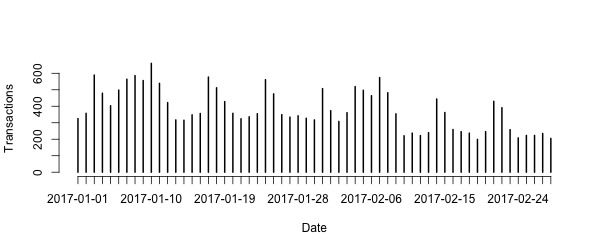
\includegraphics[width=\textwidth]{images/transbyday.png}
\end{center}
\end{frame}

\begin{frame}[fragile]{Aggregating the user-level advertising data}
We also computed the aggregate number of impressions on each day. 
\begin{lstlisting}
> (cadence <- xtabs(~date+channel, data=impress))
            channel
date         direct display email email.holdout social
  2016-12-31      0     788     0             0   1610
  2017-01-01      0    3786     0             0   7481
  2017-01-02      0    3792     0             0   7416
  2017-01-03      0    3656  4798          1203   7505
  2017-01-04      0    3731     0             0   7648
  2017-01-05      0    3770     0             0   7620
  2017-01-06   4974    3611     0             0   7614
  2017-01-07      0    3719     0             0   7552
  2017-01-08      0    3780     0             0   7504
  2017-01-09      0    3744     0             0   7446
\end{lstlisting}
\end{frame}

\begin{frame}{Advertising by day}
\begin{center}
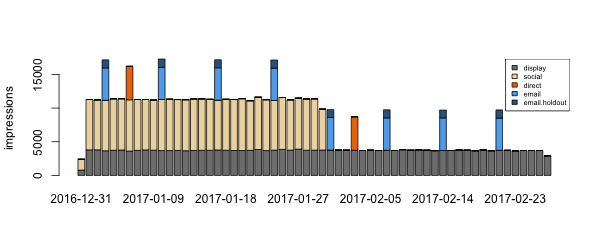
\includegraphics[width=.85\textwidth]{images/cadence.png}
\end{center}
\end{frame}

\begin{frame}[fragile]{Combining the sales and impressions data}
When we fit models, it will be convenient to put the sales and impressions data together in the same data frame. 
\begin{lstlisting}
> mdata <- as.data.frame(cbind(trans=transbyday[1:57], cadence[2:58,])) # aligining dates
> head(mdata)
           trans direct display email email.holdout social
2017-01-01   325      0    3786     0             0   7481
2017-01-02   357      0    3792     0             0   7416
2017-01-03   589      0    3656  4798          1203   7505
2017-01-04   479      0    3731     0             0   7648
2017-01-05   403      0    3770     0             0   7620
2017-01-06   498   4974    3611     0             0   7614\end{lstlisting}
\end{frame} 

\begin{frame}[fragile]{Data exploration}
Now that we have the data aggregated, we should do some exploration before modeling. 
\begin{lstlisting}
> plot(x=mdata$direct, y=mdata$trans, xlab="Direct Impressions", 
+      ylab="Transactions", main="Direct Impressions v. Transactions")
> plot(x=mdata$email, y=mdata$trans, xlab="Email Impressions", 
+      ylab="Transactions", main="Email Impressions v. Transactions")
> plot(x=mdata$display, y=mdata$trans, xlab="Display Impressions", 
+      ylab="Transactions", main="Display Impressions v. Transactions")
> plot(x=mdata$social, y=mdata$trans, xlab="Social Impressions", 
+      ylab="Transactions", main="Social Impressions v. Transactions")
\end{lstlisting}
\end{frame}

\begin{frame}{Daily display and social impressions versus transactions}
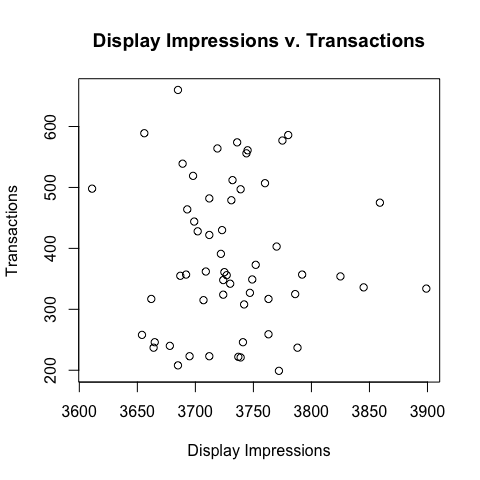
\includegraphics[width=0.5\textwidth]{images/mixmodeldisplavtrans.png}
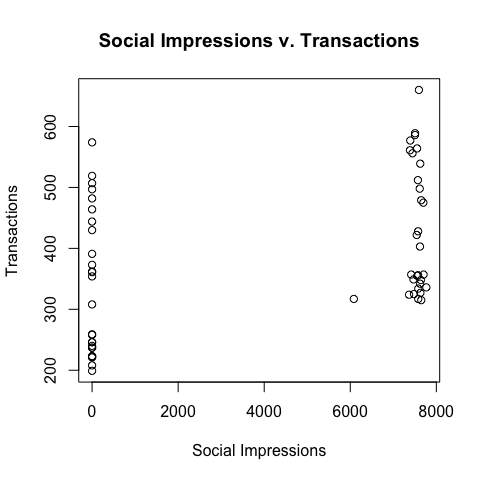
\includegraphics[width=0.5\textwidth]{images/mixmodelsocialvtrans.png}
\end{frame}

\begin{frame}{Daily email and direct mpressions versus transactions}
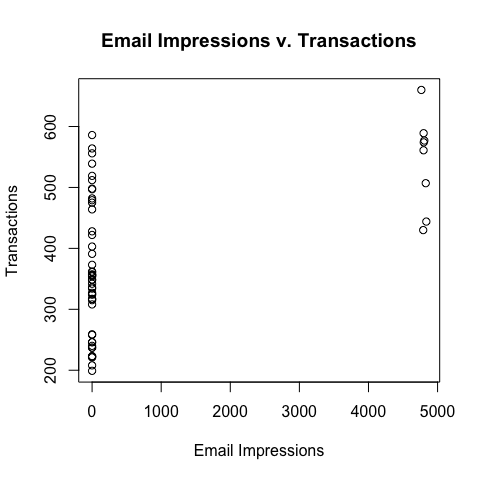
\includegraphics[width=0.5\textwidth]{images/mixmodelemailvtrans.png}
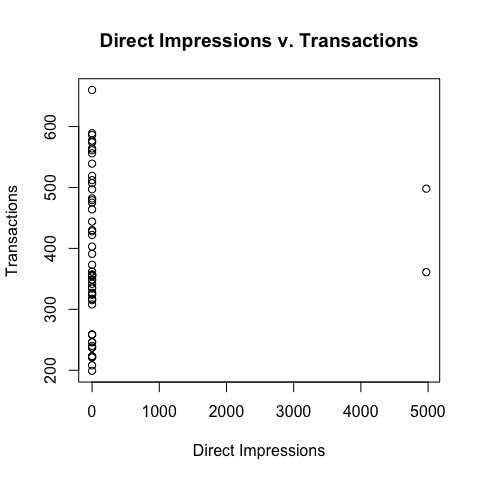
\includegraphics[width=0.5\textwidth]{images/mixmodeldirectvtrans.png}
\end{frame}

\begin{frame}[fragile]{Running a simple media mix model}
\small
\begin{lstlisting}[basicstyle=\tiny\ttfamily]
> m1 <- lm(trans~direct+social+email+display+social+email.holdout, data=mdata)
> summary(m1)
...
Coefficients:
                Estimate Std. Error t value Pr(>|t|)    
(Intercept)   438.501429 940.622551   0.466 0.643070    
direct          0.014529   0.013853   1.049 0.299206    
social          0.012663   0.003379   3.747 0.000457 ***
email          -0.161643   0.321735  -0.502 0.617541    
display        -0.035299   0.252371  -0.140 0.889313    
email.holdout   0.805475   1.290198   0.624 0.535211    
---
Signif. codes:  0 `***' 0.001 `**' 0.01 `*'0.05 `.' 0.1 ` ' 1

Residual standard error: 92.53 on 51 degrees of freedom
Multiple R-squared:  0.4644,	Adjusted R-squared:  0.4119 
F-statistic: 8.845 on 5 and 51 DF,  p-value: 0.00000427
\end{lstlisting}
\end{frame}


\begin{frame}[fragile]{Things to notice in the model output}
\begin{columns}
\column{0.5\textwidth}
\begin{lstlisting}[basicstyle=\tiny\ttfamily]
> m1 <- lm(trans~direct+social+email+display+social+email.holdout, 
           data=mdata)
> summary(m1)

Call:
lm(formula = trans ~ direct + social + email + display + social + 
    email.holdout, data = mdata)

Residuals:
    Min      1Q  Median      3Q     Max 
-106.35  -67.79  -41.56   54.42  211.04 

Coefficients:
                Estimate Std. Error t value Pr(>|t|)    
(Intercept)   438.501429 940.622551   0.466 0.643070    
direct          0.014529   0.013853   1.049 0.299206    
social          0.012663   0.003379   3.747 0.000457 ***
email          -0.161643   0.321735  -0.502 0.617541    
display        -0.035299   0.252371  -0.140 0.889313    
email.holdout   0.805475   1.290198   0.624 0.535211    
---
Signif. codes:  0 `***' 0.001 `**' 0.01 `*' 0.05 `.' 0.1 ` ' 1

Residual standard error: 92.53 on 51 degrees of freedom
Multiple R-squared:  0.4644,	Adjusted R-squared:  0.4119 
F-statistic: 8.845 on 5 and 51 DF,  p-value: 0.00000427
\end{lstlisting}
\column{0.5\textwidth}
The only statistically significant effect is for social impressions, and we get 0.012663 additional transactions for each social impression. \\
\bigskip \pause
The standard error for display is very large, which means we don't have a precise estimate of the effect of display. This happened because daily display impressions are pretty much the same every day.  The data is not informative!\\
\bigskip \pause
The estimated effect of email and display is negative (but not significant). 
\end{columns}
\end{frame}

\begin{frame}[fragile]{Adding other variables} 
In addition to advertising impressions, we might want to include other predictors of transactions in our model, such as the day of the week. 
\begin{lstlisting}
> mdata$dayofweek <- weekdays(as.Date(rownames(mdata)))
> m2 <- lm(trans~email+direct+display+social+dayofweek, data=mdata)
\end{lstlisting}
\end{frame}

\begin{frame}[fragile]{Our second model}
\begin{columns}
\column{0.55\textwidth}
\begin{lstlisting}[basicstyle=\tiny\ttfamily]
> summary(m2)

Call:
lm(formula = trans ~ email + direct + display + social + dayofweek, 
    data = mdata)

Residuals:
   Min     1Q Median     3Q    Max 
-87.09 -51.78 -21.70  25.46 221.46 

Coefficients:
                      Estimate  Std. Error t value Pr(>|t|)    
(Intercept)         348.192012  891.949059   0.390 0.698063    
email                -0.960694    1.463482  -0.656 0.514809    
direct                0.029537    0.014165   2.085 0.042632 *  
display              -0.031124    0.239069  -0.130 0.896986    
social                0.012754    0.003077   4.144 0.000145 ***
dayofweekMonday      71.405198   45.616341   1.565 0.124357    
dayofweekSaturday    64.445464   45.601326   1.413 0.164318    
dayofweekSunday      55.293919   44.598357   1.240 0.221330    
dayofweekThursday    67.663736   45.341037   1.492 0.142440    
dayofweekTuesday   4877.229334 7029.997193   0.694 0.491313    
dayofweekWednesday  171.086874   45.336050   3.774 0.000459 ***
---
Signif. codes:  0 `***' 0.001 `**' 0.01 `*' 0.05 `.' 0.1 ` ' 1

Residual standard error: 83.94 on 46 degrees of freedom
Multiple R-squared:  0.6024,	Adjusted R-squared:  0.516 
F-statistic:  6.97 on 10 and 46 DF,  p-value: 0.000001582
\end{lstlisting}
\column{0.45\textwidth}
When we add other variables, it can change the coefficients of the model.  \\
\bigskip \pause
With our new model we find a significant association between direct impressions and transactions (29.5 additional transactions / 1000 direct impressions) in addition to social (12.8 additional transactions / 1000 impressions). \\
\end{columns}
\end{frame} 

\begin{frame}{What is our model missing?}
Our story about where our data comes from says: 
\begin{equation*}
\textnormal{sales}_t = \beta_0 + \beta_1 \textnormal{display}_t + \beta_2 \textnormal{social}_t + \beta_3 \textnormal{email}_t + \beta_4 \textnormal{direct}_t + \epsilon_t
\end{equation*}\\
\bigskip \pause
Our model assumes that an impression on day $t$ has an effect on the number of transactions on day $t$ and that those impressions have no effect on sales on other days. \\
\bigskip \pause
Do we really believe that ads only work on the day they were served/sent?  \\
\bigskip \pause
Our intuition as marketers tells us this probably isn't true and our email holdout test suggests that emails last about 3 days.   
\end{frame}

\begin{frame}{Exponential decay of advertising}
\begin{columns}
\column{0.4\textwidth}
advertising effect
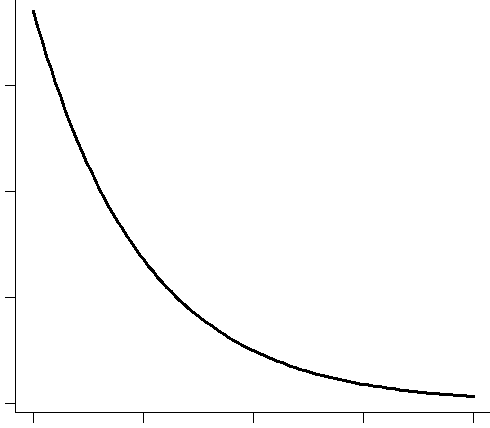
\includegraphics[width=\textwidth]{images/exponential-decay.png}
\flushright time
\column{0.6\textwidth}
One theory of advertising response is that an ad had its biggest effect just after it is shown to the user and then the effect wears off over time. \\
\bigskip \pause
We typically use an exponential decay function to describe how the effect of the ad falls off. 
\end{columns}
\end{frame}

\begin{frame}{Ad stock variables in R}
An ad stock variable is created by computing the exponential decay of the impressions on each day and then summing up the total ``stock" from impressions on previous days. The result will look something like this: \\
\begin{center}
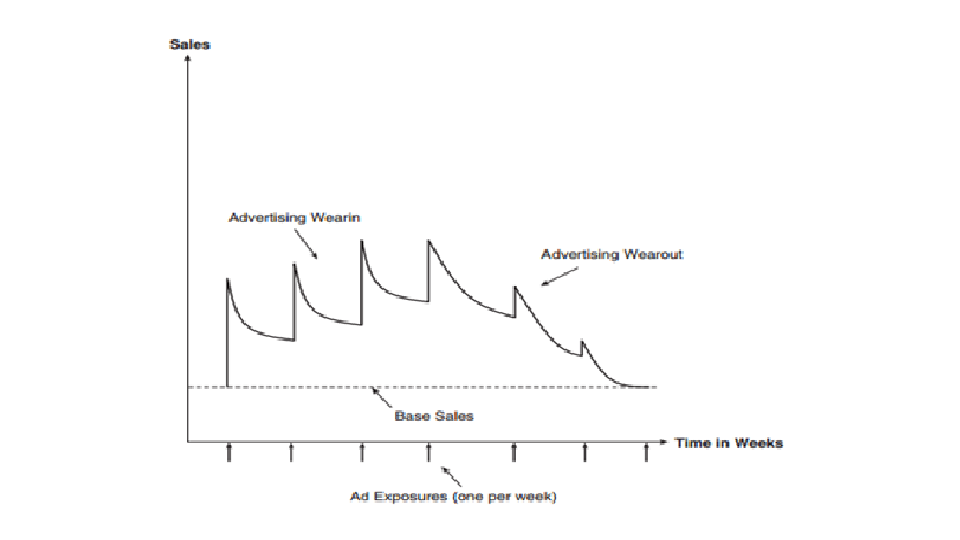
\includegraphics[width=0.6\textwidth]{images/adresponseovertime.png}
\source{\href{https://www.linkedin.com/pulse/new-tools-determining-measuring-wear-in-wear-out-media-michael-wolfe}{Michael Wolfe}}
\end{center} 
\end{frame}

\begin{frame}[fragile]{Creating ad stock variables in R}
Computing ad stock variables may sound complicated, but it is easy to do in R. 
\footnotesize
\begin{lstlisting}[basicstyle=\tiny\ttfamily]
> mdata$email.stock <- as.numeric(filter(x=mdata$email, filter=0.5, method="recursive"))
> mdata$display.stock <- as.numeric(filter(x=mdata$display, filter=0.3, method="recursive"))
> mdata$direct.stock <- as.numeric(filter(x=mdata$direct, filter=0.75, method="recursive"))
> mdata$social.stock <- as.numeric(filter(x=mdata$social, filter=0.3, method="recursive"))
\end{lstlisting}
\end{frame}

\begin{frame}[fragile]{Ad stock variables} 
\begin{lstlisting}
           trans direct display email email.holdout social dayofweek
2017-01-01   325      0    3786     0             0   7481    Sunday
2017-01-02   357      0    3792     0             0   7416    Monday
2017-01-03   589      0    3656  4798          1203   7505   Tuesday
2017-01-04   479      0    3731     0             0   7648 Wednesday
2017-01-05   403      0    3770     0             0   7620  Thursday
2017-01-06   498   4974    3611     0             0   7614    Friday
           email.stock display.stock direct.stock social.stock
2017-01-01        0.00      3786.000            0      7481.00
2017-01-02        0.00      4927.800            0      9660.30
2017-01-03     4798.00      5134.340            0     10403.09
2017-01-04     2399.00      5271.302            0     10768.93
2017-01-05     1199.50      5351.391            0     10850.68
2017-01-06      599.75      5216.417         4974     10869.20
\end{lstlisting}
\begin{center}
\alert{This might be easier with a picture.}
\end{center}
\end{frame}

\begin{frame}[fragile]{Create graphs of adstocks}
\begin{lstlisting}
> plot(mdata$email.stock, type="l", xlab="Day", ylab="Email Ad Stock")
> plot(mdata$display.stock, type="l", xlab="Day", ylab="Display Ad Stock")
> plot(mdata$direct.stock, type="l", xlab="Days", ylab="Direct Stock")
> plot(mdata$social.stock, type="l", xlab="Days", ylab="Social Stock")
\end{lstlisting}
\end{frame}

\begin{frame}{Email ad stock variable}
\begin{center}
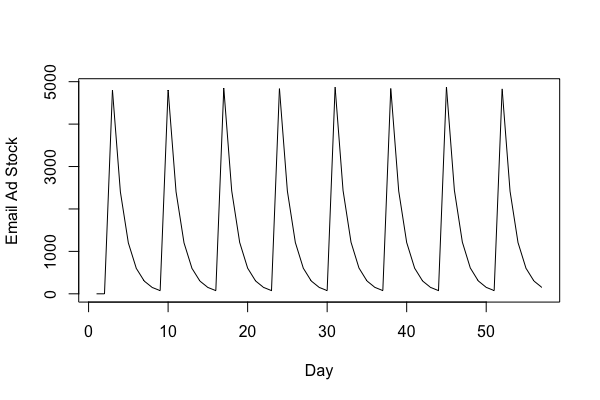
\includegraphics[width=0.7\textwidth]{images/mixmodelemailstock.png}
\end{center}
\end{frame}

\begin{frame}{Direct ad stock variable}
\begin{center}
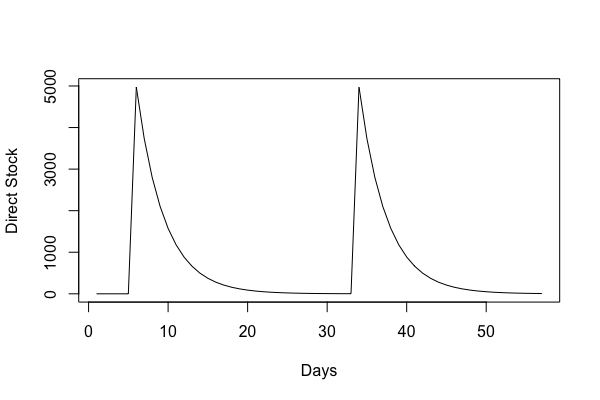
\includegraphics[width=0.7\textwidth]{images/mixmodeldirectstock.png}
\end{center}
\end{frame}

\begin{frame}{Display ad stock variable}
\begin{center}
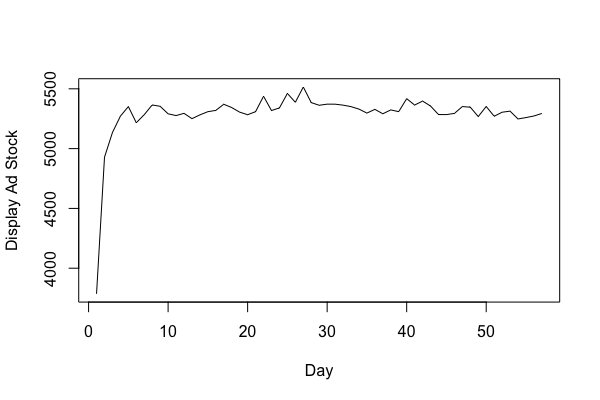
\includegraphics[width=0.7\textwidth]{images/mixmodeldisplaystock.png}
\end{center}
\end{frame}

\begin{frame}{Social ad stock variable}
\begin{center}
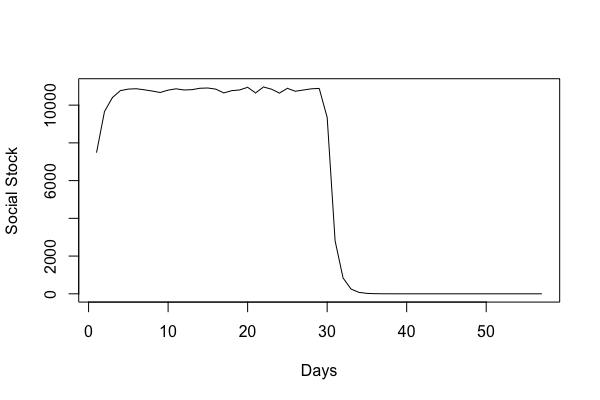
\includegraphics[width=0.7\textwidth]{images/mixmodelsocialstock.png}
\end{center}
\end{frame}

\begin{frame}[fragile]{Plot ad stock variables against transactions}
\begin{lstlisting}
> plot(mdata$email.stock, type="l", xlab="Day", ylab="Email Ad Stock")
> plot(mdata$display.stock, type="l", xlab="Day", ylab="Display Ad Stock")
> plot(mdata$direct.stock, type="l", xlab="Days", ylab="Direct Stock")
> plot(mdata$social.stock, type="l", xlab="Days", ylab="Social Stock")
\end{lstlisting}
\end{frame}

\begin{frame}{Email and direct ad stock versus transactions}
\includegraphics[width=0.5\textwidth]{images/mixmodelemailstockvtrans.png}
\includegraphics[width=0.5\textwidth]{images/mixmodeldirectstockvtrans.png}
\end{frame}

\begin{frame}{Display and social ad stock versus transactions}
\includegraphics[width=0.5\textwidth]{images/mixmodeldisplaystockvtrans.png}
\includegraphics[width=0.5\textwidth]{images/mixmodelsocialstockvtrans.png}
\end{frame}

\begin{frame}[fragile]{Marketing mix model with ad stock variables}
\begin{lstlisting}
> m3 <- lm(trans~email.stock+display.stock+direct.stock+social.stock, 
+          data=mdata[5:nrow(mdata),]) # Remove first few observations to allow for "warmup" of stock
> summary(m3)
...
Coefficients:
                 Estimate  Std. Error t value           Pr(>|t|)    
(Intercept)   -460.452735  753.753237  -0.611              0.544    
email.stock      0.050538    0.004814  10.499 0.0000000000000503 ***
display.stock    0.128309    0.141450   0.907              0.369    
direct.stock     0.055573    0.006193   8.974 0.0000000000077486 ***
social.stock     0.009468    0.001422   6.659 0.0000000245161516 ***
---
Signif. codes:  0 `***' 0.001 `**' 0.01 `*' 0.05 `.' 0.1 ` ' 1

Residual standard error: 54.17 on 48 degrees of freedom
Multiple R-squared:  0.8147,	Adjusted R-squared:  0.7992 
F-statistic: 52.74 on 4 and 48 DF,  p-value: < 0.00000000000000022
\end{lstlisting}
\end{frame}

\begin{frame}[fragile]{Things to notice about our third marketing mix model}
\begin{columns}
\column{0.5\textwidth}
\begin{lstlisting}[basicstyle=\tiny\ttfamily]
> m3 <- lm(trans~email.stock+display.stock+direct.stock+social.stock, 
+          data=mdata[5:nrow(mdata),]) 
> summary(m3)

Call:
lm(formula = trans ~ email.stock + display.stock + direct.stock + 
    social.stock, data = mdata[5:nrow(mdata), ])

Residuals:
     Min       1Q   Median       3Q      Max 
-170.442  -31.630   -3.793   19.411  125.000 

Coefficients:
                 Estimate  Std. Error t value           Pr(>|t|)    
(Intercept)   -460.452735  753.753237  -0.611              0.544    
email.stock      0.050538    0.004814  10.499 0.0000000000000503 ***
display.stock    0.128309    0.141450   0.907              0.369    
direct.stock     0.055573    0.006193   8.974 0.0000000000077486 ***
social.stock     0.009468    0.001422   6.659 0.0000000245161516 ***
---
Signif. codes:  0 `***' 0.001 `**' 0.01 `*' 0.05 `.' 0.1 ` ' 1

Residual standard error: 54.17 on 48 degrees of freedom
Multiple R-squared:  0.8147,	Adjusted R-squared:  0.7992 
F-statistic: 52.74 on 4 and 48 DF,  p-value: < 0.00000000000000022
\end{lstlisting}
\column{0.5\textwidth}
We now find positive effects for all forms of advertising. \\
\bigskip \pause
Email and display seem to have similar effects on transactions at about 50 additional transactions on the first day the piece is sent.\\
\bigskip \pause
All effects are statistically significant except for display.  Display still has a high standard error because there is not much variation in the display stock. We simply can't measure the effect of display using this data. 
\end{columns}
\end{frame}

\begin{frame}[fragile]{Estimating the decay rate}
In this example, we \alert{assumed a decay rate} for each channel when we created the ad stock variables. 
\footnotesize
\begin{lstlisting}
> mdata$email.stock <- as.numeric(filter(x=mdata$email, filter=0.5, 
                                  method="recursive"))
> mdata$display.stock <- as.numeric(filter(x=mdata$display, filter=0.3, 
                                   method="recursive"))
> mdata$direct.stock <- as.numeric(filter(x=mdata$direct, filter=0.75, 
                                   method="recursive"))
> mdata$social.stock <- as.numeric(filter(x=mdata$social, filter=0.3, 
                                   method="recursive"))
\end{lstlisting}
\normalsize
I selected a short decay rate for display and social and longer ones for email and catalog based on intuition. \alert{More sophisticated approaches estimate the decay rate from the data.}
\end{frame}

\begin{frame}{Interactions between channels}
An interaction occurs when there is an extra "boost" to having two advertising channels active at the same time. Together, the two channels are move effective than the sum of their parts. There is a synergy. \\
\bigskip \pause
We model this by adding an extra term in our model that is the multiple of two other variables. 
\begin{equation*}
\textnormal{sales}_t = \beta_0 + \beta_1 \textnormal{display}_t + \beta_2 \textnormal{social}_t + \beta_3 \textnormal{email}_t + \beta_4 \textnormal{direct}_t + \beta_5 (\textnormal{email} \times \textnormal{direct}) + \epsilon_t
\end{equation*}
This is really easy to do in R. 
\end{frame}

\begin{frame}[fragile]{Adding interactions to a model in R}
\footnotesize
\begin{lstlisting}
> m4 <-lm(trans~email.stock+display.stock+direct.stock+social.stock+
+                email.stock*direct.stock, data=mdata[5:nrow(mdata),]) 
> summary(m4)
...
                               Estimate     Std. Error t value        Pr(>|t|)    
(Intercept)              -418.432368566  764.864071866  -0.547           0.587    
email.stock                 0.052249390    0.006017106   8.683 0.0000000000248 ***
display.stock               0.120103084    0.143613018   0.836           0.407    
direct.stock                0.057597635    0.007529130   7.650 0.0000000008521 ***
social.stock                0.009506492    0.001435581   6.622 0.0000000306335 ***
email.stock:direct.stock   -0.000003204    0.000006659  -0.481           0.633    
---
Signif. codes:  0 `***' 0.001 `**' 0.01 `*''0.05 `.' 0.1 ` ' 1

Residual standard error: 54.61 on 47 degrees of freedom
Multiple R-squared:  0.8156,	Adjusted R-squared:  0.7959 
F-statistic: 41.57 on 5 and 47 DF,  p-value: 0.0000000000000003867
\end{lstlisting}
\alert{There is no significant interaction effect between email and direct mail.}
\end{frame}

\begin{frame}{Is there more to the ad response story?}
So far, we have explored a few advanced features to our model: 
\begin{itemize}
\item \alert{Ad Stock / Exponential decay}: Ads have an effect on transactions that decays over time
\item \alert{Interactions}: Ads may be synergistic
\end{itemize}
\bigskip \pause
There are several other ideas about how advertising works that we could build into a marketing mix model, but are outside the scope of this workshop: 
\begin{itemize}
\item \alert{S-shaped advertising response}
\item \alert{Wearout}
\item \alert{Competitive advertising}
\end{itemize}
\end{frame} 

\begin{frame}{S Shaped advertising response}
\begin{columns}
\column{0.5\textwidth}
\includegraphics[width=\textwidth]{images/sshapedadresponse.png}
\source{\href{https://drive.google.com/uc?export=download&id=0B0EzanlzLNsWZkE1TWtNNVpBUzA}{Little (1979)}}
\column{0.5\textwidth}
Two old saws of advertising: 
\begin{itemize} 
\item Advertising doesn't have much effect on sales until you get enough ``weight" in the market. 
\item There is a point of \alert{diminishing returns} to advertising. 
\end{itemize}
This can be modeled by assuming an ``S-shaped" advertising response curve. 
\end{columns}
\end{frame}

\begin{frame}{Wearin and wearout}
Over time, even a constant level of advertising may become less effective, particularly if the creatives don't change. 
\begin{center}
\includegraphics[width=0.7\textwidth]{images/adresponseovertime.png}
\end{center}
\source{\href{https://www.linkedin.com/pulse/new-tools-determining-measuring-wear-in-wear-out-media-michael-wolfe}{Michael Wolfe}}
\end{frame}

\begin{frame}{Little's principles}
Little (1979) summarized five key principals for marketing mix models, based on the data he had studied on aggregate advertising spending and sales. 
\includegraphics[width=\textwidth]{images/littleprincipals.png}
\source{\href{https://drive.google.com/uc?export=download&id=0B0EzanlzLNsWZkE1TWtNNVpBUzA}{Little (1979)}}
\end{frame}

% VARX Models

\subsection{What can go wrong?}

\begin{frame}[fragile]{Endogeneity bias}
If the advertiser is buying more advertising (``heaving-up") during periods she knows have high demand (like holidays), there will be a correlation between advertising and sales. \\
\bigskip \pause
This correlation will show up in our regression and we might interpret it as ``the effect of advertising", when the causality is actually reversed. \\
\bigskip \pause 
Even though our final model (\verb|m3|) seems to be giving us pretty good estimates of advertising response it might not be.  This has the terrible name \alert{endogeneity bias}.
\end{frame}

\begin{frame}{Endogeneity bias corrections}
There are some corrections for endogeneity bias in marketing mix models: 
\begin{itemize}
\item Instrumental variables
\item Model the process for setting advertising (e.g. VAR models)
\end{itemize}
\bigskip \pause
These approaches have some major drawbacks and \alert{holdout testing} is the only sure-fire way to accurately measure ad response. 
\end{frame} 

\begin{frame}{Modeler degrees of freedom}
As you have seen, there are many decisions for the modeler to make when building a marketing mix model. 
\begin{itemize}
\item Does advertising last more than one day and if so, what is the \alert{decay rate}? 
\item Should my model include \alert{diminishing returns} to the level of advertising?
\item Should my model include advertising \alert{wearout}? 
\item Should I try to \alert{correct endogeneity bias} and how? 
\end{itemize}
\bigskip \pause
The problem with having so many modeling choices is that it is tempting to keep trying different models until you find the one that you (or your client) like. This is sometimes called the \alert{garden of forking paths} and it is a dangerous place for an analyst to be! You may end up with a model you like rather than one that is right. 
\end{frame}

\begin{frame}{Summary: marketing mix models}
A \alert{marketing mix model} is a \alert{regression} relating advertising spending or total impressions to some response like sales. \\
\bigskip
To build a marketing mix model, you assemble data on advertising spending or impressions by day/week/month and conversions or sales by day/week/month and then fit a model using any regression tool.   \\
\bigskip
The coefficients of this model tell us the correlations between daily/weekly/monthly levels of advertising and sales.\\
\end{frame}

\begin{frame}{What can go wrong with marketing mix modeling?}
There isn't enough variation in the advertising over time or two different types of advertising tend to happen at the same time. \\
\begin{itemize}
\item Model estimates will show large standard errors on the coefficients.  You'll be stuck, but at least you'll know it. 
\end{itemize}
\pause
Advertising happens during periods of peak demand, reversing the causality. \\
\begin{itemize}
\item Model estimates may appear reasonable but will overestimate advertising response.  You'll be wrong, but you won't know it. 
\end{itemize}
\pause 
The analyst can twittle with the model until she gets it to say what she likes or what you want to hear. 
\end{frame} 

\section{Model-based attribution}

\subsection{What is model-based attribution?}

\begin{frame}{Model-based attribution}
\alert{Model-based attribution} is similar to marketing mix modeling, but we do the analysis at the user-level, relating a user's transactions or conversions to her prior advertising exposures.  A simple attribution model is: 
\begin{equation*}
conversion_{it} = \beta_0 + \beta_1 \textnormal{display}_{it} + \beta_2 \textnormal{social}_{it} + \beta_3 \textnormal{email}_{it} + \beta_4 \textnormal{direct}_{it} + \epsilon_{it}
\end{equation*} 
The key difference from a marketing mix model is that now all the variables are \alert{indexed by $i$} in addition to $t$.
\end{frame}

\subsection{Model-based attribution in R}

\begin{frame}[fragile]{Model-based attribution in R}
To run this regression, we need to create a data frame where each row is a user-day and summarizes the user's impressions and transactions on that day. We have to transform the raw data to this: 
\footnotesize
\begin{lstlisting}[basicstyle=\tiny\ttfamily]
> head(adata)
  id       date direct display email email.holdout social trans past.purchase has.email has.direct
1  1 2017-01-01      0       0     0             0      1     0             0         0          1
2  1 2017-01-02      0       0     0             0      1     0             0         0          1
3  1 2017-01-03      0       0     0             0      0     0             0         0          1
4  1 2017-01-04      0       0     0             0      0     0             0         0          1
5  1 2017-01-05      0       0     0             0      1     0             0         0          1
6  1 2017-01-06      1       0     0             0      2     0             0         0          1
\end{lstlisting}
My R code for doing this is a bit messy and takes several steps. I'm sure you could do better with \href{https://blog.rstudio.org/2016/09/15/tidyverse-1-0-0/}{tidyverse}.
\end{frame}

\begin{frame}[fragile]{Data transform step 1: Summary of impressions by user and day}
\footnotesize
First, we create a data frame that has a daily summary of each user's transactions. 
\begin{lstlisting}[basicstyle=\tiny\ttfamily]
> adatal <- as.data.frame(xtabs(~ id + date + channel, data=impress), stringsAsFactors=FALSE)
> adatal$id <- as.integer(adatal$id)
> adatal$date <- as.Date(adatal$date)
> adatal$channel <- as.factor(adatal$channel)
> dimnames(adatal)[[2]][4] <- "impr"
> head(adatal)
  id       date channel impr
1  1 2016-12-31  direct    0
2  2 2016-12-31  direct    0
3  3 2016-12-31  direct    0
4  5 2016-12-31  direct    0
5  6 2016-12-31  direct    0
6  7 2016-12-31  direct    0
\end{lstlisting}
\end{frame}

\begin{frame}[fragile]{Data transform step 2: Adding in users with zero impressions}
\footnotesize
Because some users don't appear in the impressions file, we have to add in rows (with zeros) for those 
users.
\begin{lstlisting}[basicstyle=\tiny\ttfamily]
> pop <- unique(cust$id)
> no.impress.ids <- pop[!(pop %in% unique(impress$id))]
> dates <- sort(unique(impress$date))
> channels <- unique(impress$channel)
> no.impress.obs <- data.frame(id=rep(no.impress.ids, each=length(dates)*length(channels)), 
+                              date=rep(rep(dates, each=length(channels)), length(no.impress.ids)), 
+                              channel=rep(channels, length(no.impress.ids)*length(dates)),
+                              impr=rep(0, length(dates)*length(no.impress.ids)*length(channels)), 
+                              stringsAsFactors=FALSE)
> no.impress.obs$channel <- as.factor(no.impress.obs$channel)
> adatal <- rbind(adatal, no.impress.obs)
> summary(adatal)
       id             date                     channel            impr        
 Min.   :    1   Min.   :2016-12-31   direct       :590000   Min.   : 0.0000  
 1st Qu.: 2501   1st Qu.:2017-01-14   display      :590000   1st Qu.: 0.0000  
 Median : 5000   Median :2017-01-29   email        :590000   Median : 0.0000  
 Mean   : 5000   Mean   :2017-01-29   email.holdout:590000   Mean   : 0.1699  
 3rd Qu.: 7500   3rd Qu.:2017-02-13   social       :590000   3rd Qu.: 0.0000  
 Max.   :10000   Max.   :2017-02-27                          Max.   :16.0000  
\end{lstlisting}
\end{frame}

\begin{frame}[fragile]{Data transform step 3: Switch to wide format}
\footnotesize
Next, we unstack the impressions column by the channel.
\begin{lstlisting}[basicstyle=\tiny\ttfamily]
> adata <- reshape(adatal, direction="wide", v.names="impr", idvar=c("id", "date"), 
+                 timevar="channel", new.row.names=NULL)
> sum(adata$impr.direct) == length(impress$channel[impress$channel=="direct"]) #quick check
[1] TRUE
> nrow(adata)
[1] 590000
> head(adata)
  id       date impr.direct impr.display impr.email impr.email.holdout impr.social
1  1 2016-12-31           0            0          0                  0           0
2  2 2016-12-31           0            0          0                  0           0
3  3 2016-12-31           0            0          0                  0           0
4  5 2016-12-31           0            1          0                  0           0
5  6 2016-12-31           0            0          0                  0           0
6  7 2016-12-31           0            0          0                  0           0
\end{lstlisting}
\end{frame}

\begin{frame}[fragile]{Data transformation step 4: Add the daily transactions for each user}
Finally, we summarize the transactions by customer-day and merge with impressions.
\begin{lstlisting}[basicstyle=\tiny\ttfamily]
> atrans <- as.data.frame(xtabs(~ id + date, data=trans), stringsAsFactors=FALSE)
> atrans$id <- as.integer(atrans$id)
> atrans$date <- as.Date(atrans$date)
> dimnames(atrans)[[2]][3] <- "trans"
> adata <- merge(adata, atrans, by=c("id", "date"), all=TRUE)
> adata$trans[is.na(adata$trans)] <- 0  # fill in zeros for transactions
> head(adata)
  id       date impr.direct impr.display impr.email impr.email.holdout impr.social trans
1  1 2016-12-31           0            0          0                  0           0     0
2  1 2017-01-01           0            0          0                  0           1     0
3  1 2017-01-02           0            0          0                  0           1     0
4  1 2017-01-03           0            0          0                  0           0     0
5  1 2017-01-04           0            0          0                  0           0     0
6  1 2017-01-05           0            0          0                  0           1     0
\end{lstlisting}
\end{frame}

\begin{frame}[fragile]{Data transformation step 5: Final tidy up of attribution modeling data}
\footnotesize
\begin{lstlisting}[basicstyle=\tiny\ttfamily]
> # Remove first and last days (which are incomplete)
> adata <- adata[adata$date!="2016-12-31" & adata$date != "2017-02-28" & adata$date != "2017-02-27",] 
# Add customer info from cust table
> adata <- merge(adata, cust, by=c("id"))
# Tidy up column names
> dimnames(adata)[[2]][3:11] <- c("direct", "display", "email", "email.holdout", "social", 
               "trans", "past.purchase", "has.email", "has.direct")
> rm(adatal, atrans)
\end{lstlisting}
\end{frame}

\begin{frame}[fragile]{Summary of attribution modeling data}
\footnotesize
\begin{lstlisting}[basicstyle=\tiny\ttfamily]
> summary(adata)
       id             date                direct           display            email        
 Min.   :    1   Min.   :2017-01-01   Min.   :0.00000   Min.   : 0.0000   Min.   :0.00000  
 1st Qu.: 2501   1st Qu.:2017-01-15   1st Qu.:0.00000   1st Qu.: 0.0000   1st Qu.:0.00000  
 Median : 5000   Median :2017-01-29   Median :0.00000   Median : 0.0000   Median :0.00000  
 Mean   : 5000   Mean   :2017-01-29   Mean   :0.01745   Mean   : 0.3731   Mean   :0.06741  
 3rd Qu.: 7500   3rd Qu.:2017-02-12   3rd Qu.:0.00000   3rd Qu.: 0.0000   3rd Qu.:0.00000  
 Max.   :10000   Max.   :2017-02-26   Max.   :1.00000   Max.   :13.0000   Max.   :1.00000  
 email.holdout         social            trans         past.purchase      has.email     
 Min.   :0.00000   Min.   : 0.0000   Min.   :0.00000   Min.   :0.0000   Min.   :0.0000  
 1st Qu.:0.00000   1st Qu.: 0.0000   1st Qu.:0.00000   1st Qu.:0.0000   1st Qu.:0.0000  
 Median :0.00000   Median : 0.0000   Median :0.00000   Median :1.0000   Median :1.0000  
 Mean   :0.01681   Mean   : 0.3954   Mean   :0.03858   Mean   :0.5022   Mean   :0.6001  
 3rd Qu.:0.00000   3rd Qu.: 0.0000   3rd Qu.:0.00000   3rd Qu.:1.0000   3rd Qu.:1.0000  
 Max.   :1.00000   Max.   :16.0000   Max.   :1.00000   Max.   :1.0000   Max.   :1.0000  
   has.direct    
 Min.   :0.0000  
 1st Qu.:0.0000  
 Median :0.0000  
 Mean   :0.4974  
 3rd Qu.:1.0000  
 Max.   :1.0000  
\end{lstlisting}
\end{frame}

\begin{frame}[fragile]{Summary of attribution modeling data on a specific day}
\footnotesize
\begin{lstlisting}[basicstyle=\tiny\ttfamily]
> summary(adata[adata$date=="2017-01-03",])
       id             date                direct     display           email        email.holdout   
 Min.   :    1   Min.   :2017-01-03   Min.   :0   Min.   :0.0000   Min.   :0.0000   Min.   :0.0000  
 1st Qu.: 2501   1st Qu.:2017-01-03   1st Qu.:0   1st Qu.:0.0000   1st Qu.:0.0000   1st Qu.:0.0000  
 Median : 5000   Median :2017-01-03   Median :0   Median :0.0000   Median :0.0000   Median :0.0000  
 Mean   : 5000   Mean   :2017-01-03   Mean   :0   Mean   :0.3656   Mean   :0.4798   Mean   :0.1203  
 3rd Qu.: 7500   3rd Qu.:2017-01-03   3rd Qu.:0   3rd Qu.:0.0000   3rd Qu.:1.0000   3rd Qu.:0.0000  
 Max.   :10000   Max.   :2017-01-03   Max.   :0   Max.   :9.0000   Max.   :1.0000   Max.   :1.0000  
     social            trans        past.purchase      has.email        has.direct    
 Min.   : 0.0000   Min.   :0.0000   Min.   :0.0000   Min.   :0.0000   Min.   :0.0000  
 1st Qu.: 0.0000   1st Qu.:0.0000   1st Qu.:0.0000   1st Qu.:0.0000   1st Qu.:0.0000  
 Median : 0.0000   Median :0.0000   Median :1.0000   Median :1.0000   Median :0.0000  
 Mean   : 0.7505   Mean   :0.0589   Mean   :0.5022   Mean   :0.6001   Mean   :0.4974  
 3rd Qu.: 1.0000   3rd Qu.:0.0000   3rd Qu.:1.0000   3rd Qu.:1.0000   3rd Qu.:1.0000  
 Max.   :12.0000   Max.   :1.0000   Max.   :1.0000   Max.   :1.0000   Max.   :1.0000  
\end{lstlisting}
\end{frame}

\begin{frame}[fragile]{Visualizing the relationship between impressions and transactions}
\footnotesize
\begin{lstlisting}
> plot(aggregate(trans~direct, data=adata, FUN=mean), type="h", ylim=c(0,0.15),
+      xlab="Impressions on Day", ylab="Same-Day Conversion Rate", main="Direct")
> plot(aggregate(trans~email, data=adata, FUN=mean), type="h", ylim=c(0,0.15),
+      xlab="Impressions on Day", ylab="Same-Day Conversion Rate", main="Email")
> plot(aggregate(trans~display, data=adata, FUN=mean), type="h", ylim=c(0,0.15),
+      xlab="Impressions on Day", ylab="Same-Day Conversion Rate", main="Display")
> plot(aggregate(trans~social, data=adata, FUN=mean), type="h", ylim=c(0,0.15),
+      xlab="Impressions on Day", ylab="Same-Day Conversion Rate", main="Social")
\end{lstlisting}
\end{frame}

\begin{frame}{Direct and email daily impressions versus transactions}
\includegraphics[width=0.45\textwidth]{images/attribmodelemailvtrans.png}
\includegraphics[width=0.45\textwidth]{images/attribmodeldirectvtrans.png}\\
\alert{Looking at user-level data, it is easy to see that users convert more on days they get emails or direct mail.}
\end{frame}

\begin{frame}{Display and social daily impressions versus transactions}
\includegraphics[width=0.45\textwidth]{images/attribmodeldisplayvtrans.png}
\includegraphics[width=0.45\textwidth]{images/attribmodelsocialvtrans.png}
\end{frame}

\begin{frame}[fragile]{A simple attribution model}
\begin{lstlisting}
> m1 <- lm(trans ~ direct + display + email + social, data=adata)
> summary(m1)
...
Coefficients:
             Estimate Std. Error t value            Pr(>|t|)    
(Intercept) 0.0296060  0.0003024   97.91 <0.0000000000000002 ***
direct      0.0306548  0.0019423   15.78 <0.0000000000000002 ***
display     0.0041618  0.0002759   15.09 <0.0000000000000002 ***
email       0.0520472  0.0010144   51.31 <0.0000000000000002 ***
social      0.0085516  0.0002542   33.64 <0.0000000000000002 ***
---
Signif. codes:  0 `***' 0.001 `**' 0.01 `*' 0.05 `.' 0.1 ` ' 1

Residual standard error: 0.1919 on 569995 degrees of freedom
Multiple R-squared:  0.007249,	Adjusted R-squared:  0.007242 
F-statistic:  1041 on 4 and 569995 DF,  p-value: < 0.00000000000000022
\end{lstlisting}
\end{frame}

\begin{frame}[fragile]{Key things to notice about our attribution model}
\begin{columns}[t]
\column{0.55\textwidth}
\begin{lstlisting}[basicstyle=\tiny\ttfamily]
> m1 <- lm(trans ~ direct + display + email + social, data=adata)
> summary(m1)
...
Coefficients:
             Estimate Std. Error t value            Pr(>|t|)    
(Intercept) 0.0296060  0.0003024   97.91 <0.0000000000000002 ***
direct      0.0306548  0.0019423   15.78 <0.0000000000000002 ***
display     0.0041618  0.0002759   15.09 <0.0000000000000002 ***
email       0.0520472  0.0010144   51.31 <0.0000000000000002 ***
social      0.0085516  0.0002542   33.64 <0.0000000000000002 ***
---
Signif. codes:  0 `***' 0.001 `**' 0.01 `*' 0.05 `.' 0.1 ` ' 1

Residual standard error: 0.1919 on 569995 degrees of freedom
Multiple R-squared:  0.007249,	Adjusted R-squared:  0.007242 
F-statistic:  1041 on 4 and 569995 DF,  p-value: < 0.00000000000000022
\end{lstlisting}
\column{0.45\textwidth}
We have gotten reasonable estimates of advertising response even for this simple model that only looks at same-day response. For example, 1 email impressions is associated with 0.052 additional transactions on the same day. \\
\bigskip \pause
The probability of transacting on a day where the user is exposed to no advertising is ~3\%.  It would be bad to assume that all sales are due to advertising. 
\end{columns}
\end{frame}

\begin{frame}[fragile]{A model that includes user-characteristics}
Because we have a user-level model, we can bring in user characteristics. 
\begin{lstlisting}
> m2 <- lm(trans ~ direct + display + email + social + past.purchase, data=adata)
> summary(m2)
Coefficients:
               Estimate Std. Error t value            Pr(>|t|)    
(Intercept)   0.0142352  0.0003889   36.60 <0.0000000000000002 ***
direct        0.0203596  0.0019427   10.48 <0.0000000000000002 ***
display       0.0041846  0.0002749   15.22 <0.0000000000000002 ***
email         0.0433566  0.0010205   42.49 <0.0000000000000002 ***
social        0.0086049  0.0002533   33.97 <0.0000000000000002 ***
past.purchase 0.0320725  0.0005130   62.52 <0.0000000000000002 ***
---
Signif. codes:  0 `***' 0.001 `**' 0.01 `*' 0.05 `.' 0.1 ` ' 1

Residual standard error: 0.1912 on 569994 degrees of freedom
Multiple R-squared:  0.01401,	Adjusted R-squared:  0.014 
F-statistic:  1620 on 5 and 569994 DF,  p-value: < 0.00000000000000022
\end{lstlisting}
\end{frame}

\begin{frame}[fragile]{A model that includes user-characteristics}
\begin{columns}[t]
\column{0.55\textwidth}
\begin{lstlisting}[basicstyle=\tiny\ttfamily]
> m2 <- lm(trans ~ direct + display + email + social + 
>                 past.purchase, data=adata)
> summary(m2)
Coefficients:
               Estimate Std. Error t value            Pr(>|t|)    
(Intercept)   0.0142352  0.0003889   36.60 <0.0000000000000002 ***
direct        0.0203596  0.0019427   10.48 <0.0000000000000002 ***
display       0.0041846  0.0002749   15.22 <0.0000000000000002 ***
email         0.0433566  0.0010205   42.49 <0.0000000000000002 ***
social        0.0086049  0.0002533   33.97 <0.0000000000000002 ***
past.purchase 0.0320725  0.0005130   62.52 <0.0000000000000002 ***
---
Signif. codes:  0 `***' 0.001 `**' 0.01 `*' 0.05 `.' 0.1 ` ' 1

Residual standard error: 0.1912 on 569994 degrees of freedom
Multiple R-squared:  0.01401,	Adjusted R-squared:  0.014 
F-statistic:  1620 on 5 and 569994 DF,  p-value: < 0.00000000000000022
\end{lstlisting}
\column{0.45\textwidth}
The model suggests that customers who have not made a purchase before are much less likely to make a purchase (1.4\% versus 4.6\% baseline rate without advertising). \\
\bigskip \pause
The estimates of advertising effects are smaller than in our first model. This is because people who have made a purchase are more likely to be exposed to advertising. When we control for past purchase, we can see that the effects of advertising are smaller than we might have thought based on the first model. \\
\bigskip \pause
\alert{The controls you choose to add to the model can be critical.}
\end{columns}
\end{frame}

\begin{frame}{Logistic regression}
Those of you who learned regression from a careful teacher may have noticed that I was violating a key assumption of the linear regression model. \\
\bigskip \pause
Our outcome variable is binary and so it would be better to use a logistic regression for binary outcomes.
\end{frame}

\begin{frame}[fragile]{Logistic regression for attribution}
\footnotesize
\begin{lstlisting}
> m3 <- glm(trans ~ direct + display + email + social + past.purchase, 
+           family=binomial(), data=adata)
> summary(m3)
...
Coefficients:
               Estimate Std. Error  z value            Pr(>|z|)    
(Intercept)   -4.022893   0.014013 -287.078 <0.0000000000000002 ***
direct         0.412554   0.041688    9.896 <0.0000000000000002 ***
display        0.100630   0.006581   15.291 <0.0000000000000002 ***
email          0.762355   0.020010   38.099 <0.0000000000000002 ***
social         0.180079   0.005356   33.621 <0.0000000000000002 ***
past.purchase  0.957207   0.015672   61.079 <0.0000000000000002 ***
---
Signif. codes:  0 `***' 0.001 `**' 0.01 `*' 0.05 `.' 0.1 ` ' 1

(Dispersion parameter for binomial family taken to be 1)

    Null deviance: 186297  on 569999  degrees of freedom
Residual deviance: 178869  on 569994  degrees of freedom
AIC: 178881

Number of Fisher Scoring iterations: 6
\end{lstlisting}
\end{frame}

\begin{frame}[fragile]{Logistic regression for attribution}
\begin{columns}[t]
\column{0.55\textwidth}
\begin{lstlisting}[basicstyle=\tiny\ttfamily]
> m3 <- glm(trans ~ direct + display + email + social + past.purchase, 
+           family=binomial(), data=adata)
> summary(m3)
...
Coefficients:
               Estimate Std. Error  z value            Pr(>|z|)    
(Intercept)   -4.022893   0.014013 -287.078 <0.0000000000000002 ***
direct         0.412554   0.041688    9.896 <0.0000000000000002 ***
display        0.100630   0.006581   15.291 <0.0000000000000002 ***
email          0.762355   0.020010   38.099 <0.0000000000000002 ***
social         0.180079   0.005356   33.621 <0.0000000000000002 ***
past.purchase  0.957207   0.015672   61.079 <0.0000000000000002 ***
---
Signif. codes:  0 `***' 0.001 `**' 0.01 `*' 0.05 `.' 0.1 ` ' 1

(Dispersion parameter for binomial family taken to be 1)

    Null deviance: 186297  on 569999  degrees of freedom
Residual deviance: 178869  on 569994  degrees of freedom
AIC: 178881

Number of Fisher Scoring iterations: 6
\end{lstlisting}
\column{0.45\textwidth}
While this model is better, the logistic regression coefficients can be difficult to interpret. \\
\bigskip \pause
We are still seeing that direct and email have a bigger effect than a single display or social impression.
\end{columns}
\end{frame}

\subsection{Advanced attribution model features}

\begin{frame}{Advanced attribution modeling features}
\begin{itemize}
\item \alert{Ad stock decay} 
\begin{itemize}
\item Similar to marketing mix models
\end{itemize}
\item \alert{Wearout} 
\begin{itemize}
\item Can model reduced effectiveness of ads at the user level
\end{itemize}
\item \alert{Interactions between channels} 
\begin{itemize}
\item Similar to marketing mix models
\end{itemize}\item \alert{User differences} in advertising response (\alert{heterogeneity})
\begin{itemize}
\item Individual-level parameters for ad response can be used to target customers
\end{itemize}
\item \alert{Endogeneity bias corrections}
\begin{itemize}
\item More and better options than in marketing mix
\end{itemize}
\end{itemize}
\pause
These are all things you should ask about when assessing an attribution provider. \alert{Many commercial attribution solutions are lacking one or more of these features.}
\end{frame}

\begin{frame}{User differences in advertising response (heterogeneity)}
The models we have estimated have assumed that the effect of advertising is the same for all users.  This can't possibly be true. \\
\bigskip \pause
More advanced attribution models allow for differences between users in advertising response. 
\begin{equation*}
conversion_{it} = \beta_{0t} + \beta_{1t} \textnormal{display}_{it} + \beta_{2t} \textnormal{social}_{it} + \beta_{3t} \textnormal{email} + \beta_{4t} \textnormal{direct} + \epsilon_{it}
\end{equation*}
\begin{center}
\alert{The key addition here is the $t$ subscript on the $\beta$s.} 
\end{center}
\end{frame} 

\begin{frame}{Ad stock at the individual-level}
The ad stock concept makes a lot of sense when it is computed at the user-level.  Goodwill toward the brand is a function of the previous impression that \emph{an individual user} has received.  
\begin{center}
\includegraphics[width=0.6\textwidth]{images/adresponseovertime.png}
\end{center} 
\source{\href{https://www.linkedin.com/pulse/new-tools-determining-measuring-wear-in-wear-out-media-michael-wolfe}{Michael Wolfe}}
\end{frame}

% todo: Braun and Moe (2013) should be expanded into an example
\begin{frame}{Effects of individual creatives: wearout}
\begin{columns}
\column{0.5\textwidth}
\includegraphics[width=\textwidth]{images/ad_stock_over_time.png}
\source{Working version of \href{https://drive.google.com/uc?export=download&id=0B0EzanlzLNsWRHZ6bFh6aHZXQ28}{Braun and Moe (2013)}}
\column{0.5\textwidth}
Focusing on display ads only, Moe and Braun (2013) propose a model that includes: 
\begin{itemize}
\item Different effects for each creative
\item Wearout effects: the effect of a creative is a function of how long it has been since the user has last seen that creative
\end{itemize}
This type of model can be used to plan ad rotations.\\
\bigskip
This model is described in detail in \href{https://drive.google.com/uc?export=download&id=0B0EzanlzLNsWRHZ6bFh6aHZXQ28}{Braun and Moe (2013) Online Display Advertising: Modeling the Effects of Multiple Creatives and Individual Impression Histories}.
\end{columns}
\end{frame}

\begin{frame}{Endogeneity bias corrections in attribution models}
We have more and better options for endogeneity bias corrections in attribution models: 
\begin{itemize}
\item Bring good user-level control variables into the model. 
\item Select a set of non-exposed users who ``look similar" to those who were exposed (e.g. \alert{propensity score matching}). 
\item If there was a sharp cutoff for those who did and did not receive the advertising, you can compare those just above to those just below the threshold (called \alert{regression discontinuity}).
\end{itemize}
\alert{You should ask attribution vendors to explain their approach to correcting endogeneity bias.} 
\end{frame}

\subsection{Example: Zantedeschi, Feit and Bradlow (2017)}

\begin{frame}{Example: catalog and email response for an online retailer}
\begin{columns}
\column{0.15\textwidth}
\begin{center}
\includegraphics[width=\textwidth]{images/Subscribe.jpeg} \\
\bigskip
\includegraphics[width=1.2\textwidth]{images/Catalog_Icon.jpg}
\end{center}
\column{0.85\textwidth}
\begin{itemize}
\item 300 customers from the the retailer's CRM system
\begin{itemize}
\item E-mails sent to each customer
\item Catalogs sent to each customer
\item Daily purchase amount (direct/in-store) for each customer
\begin{itemize}
\item $>$ 90\% of transactions can be matched to an existing customer by name, credit card, etc.
\end{itemize}
\end{itemize}
\item Observations from 1 April 2012 to 10 May 2014
\item All of these customers were targeted in each campaign, but sometimes were included in a holdout test
\end{itemize}
\end{columns}
\bigskip \pause
This attribution model is reported in \href{https://drive.google.com/uc?export=download&id=0B0EzanlzLNsWRWZxVTNnZlFsUGc}{Zantedeschi, Feit and Bradlow (2017) Measuring multi-channel advertising response, \emph{Management Science}, forthcoming.} 
\end{frame}

\begin{frame}{Why not marketing mix modeling?}
\begin{columns}[T]
\column{0.5\textwidth}
\includegraphics[height=0.5\textheight]{images/campaigns_by_day.pdf} \\
\includegraphics[height=0.5\textheight]{images/sales_by_day.pdf}
\column{0.5\textwidth}
\begin{itemize}
\item As is common in direct marketing, the cadence and reach of campaigns is very steady over time. 
\item Sales are also quite steady over time. 
\item Lack of variation makes it difficult to determine any relationship between sales and marketing from aggregate data.
\end{itemize}
\end{columns}
\end{frame}

\begin{frame}{Customer-level advertising response data}
\begin{center}
\includegraphics[width=0.8\textwidth]{images/cust_143.pdf} \\
\end{center}
\end{frame}

\begin{frame}{Analyzing campaigns as individual field experiments}
Each holdout test can be analyzed individually.\\
\bigskip
\footnotesize
July 2012 Catalog Campaign
\begin{center}
\begin{tabular}{ccccc}
  \hline
 & Customers  & Ave.  & 30-Day  & Ave. \\ 
 & (N) & 30-Day & Purchase & Prior 30-Day \\
 & & Sales (\$) & Incidence & Sales (\$) \\
  \hline
 Treated & 284 & 62.34 & 0.25 & 58.82 \\ 
  Holdout &  16 & 11.90 & 0.06 & 62.65 \\ 
  \hline
  Difference &  & 50.44 & 0.18 & -3.84 \\ 
  95\% CI &  & (18.95, 81.92) & (0.04, 1) & (-91.82, 84.13) \\ 
   \hline
\end{tabular}
\end{center}
\end{frame}

\begin{frame}{Attribution model features}
Differences in advertising response across customers (heterogeneity)\\
\bigskip
A tobit model for purchase amount (\$) \\
\bigskip
Estimated decay rates for catalog and emails\\
\bigskip
Interaction between email and catalog\\
\bigskip
No endogeneity correction (We don't need it, as all exposure were randomized in holdout test)
\end{frame}

\begin{frame}[t]
\frametitle{A multi-channel, consumer-level ad-stock model}
We relate the weekly total purchase amount, $Y_{it}$, for each user $i$ in each period $t$ to the advertising exposures, $X_{ikt}$, on each channel $k$ in all previous periods as follows:
\begin{columns}
\column{0.8\textwidth}
\begin{align*}
\alert<2>{Y_{it}} &= \left \{
\begin{array}{l l}
\alert<2>{Y^{\ast}_{it}} & \alert<2>{\text{if } Y^{\ast}_{it}>0}\\
\alert<2>{0} & \alert<2>{\text{if } Y^{\ast}_{it} \le 0} \\
\end{array}
\right . \\
Y^{\ast}_{it} &= \alert<5>{\mu_i} + \alert<3>{\sum_{k}\alert<5>{\beta_{ik}} W_{ikt}} + \alert<4>{\sum_{k:k'}\alert<5>{\beta_{i,k:k'}} \alert<4>{W_{i,k:k',t}}} +  \eta_{it} \\ %\alert<3>{\alert<4>{\gamma_i}V_{ikt}}+
\alert<3>{W_{ikt}} &= \alert<3>{\sum_{s=0}^{\infty}\alert<5>{\rho_{ik}}^s (X_{i,k,t-s} + \epsilon_{ikt})} \\
\alert<4>{W_{i,k:k',t}} &= \alert<4>{\sum_{s=0}^{\infty}\alert<5>{\rho_{i,k:k'}}^s (X_{i,k,t-s}+X_{i,k,t-s} + \epsilon_{ikt})} \\
%\alert<4>{V_{it}} &= \alert<3>{\sum_{j=0}^{\infty}\alert<4>{\delta_{i}}^s  \textbf{1}\left[Y_{i,t-s}>0 \right] + \nu_{it}} \\ 
\end{align*}
\column{0.3\textwidth}
\footnotesize
\onslide<2>{\begin{block}{} \centering Tobit I selection \end{block}}
\onslide<3>{\begin{block}{} \centering Channel-specific stocks\end{block}} 
\onslide<4>{\begin{block}{} \centering Interactions \end{block}} 
\onslide<5>{\begin{block}{} \centering Heterogeneity \end{block}} 
%\alert<6>{State dependence} \\
\end{columns}
\end{frame}

\begin{frame}
\frametitle{Catalog versus email impulse response}
\begin{columns}
\column[T]{0.5\textwidth}
\centering
\includegraphics[width=\textwidth]{images/CIR_CAT_EMAIL2.pdf} \\
\column[T]{0.5\textwidth}
\footnotesize
Simulating the total incremental sales gained by sending each customer a catalog during the first week of the year versus e-mail, we find that catalog is slightly more effective than e-mail. \\
\end{columns}
\end{frame}

\begin{frame}
\frametitle{Combined catalog and email impulse response}
\begin{columns}
\column[T]{0.5\textwidth}
\centering
\includegraphics[width=\textwidth]{images/CIR_CUM_PLOT_2.pdf} \\
\column[T]{0.5\textwidth}
\footnotesize
Sending both an email and a catalog during the same week produces additional incremental sales lift.\\
\end{columns}
\end{frame}

\section{Review}

\begin{frame}{Why not search ads?}
\begin{columns}
\column{0.5\textwidth}
\includegraphics[width=\textwidth]{images/searchad.png}
\column{0.5\textwidth}
You may have noticed that our example didn't include search advertising and I didn't talk about search except for the search geo-test.\\
\bigskip \pause
\begin{center} \alert{Why?} \end{center}
\bigskip \pause
Google doesn't report search ad impressions for individual users (only clicks).  We can include search clicks in our attribution models as an ``impression", but they aren't really impressions. There is heavy self-selection in who clicks on a search ad. 
\end{columns}
\end{frame}

\begin{frame}{Methods for estimating advertising response}
\footnotesize
\begin{tabular}{l l l}
Method & Pros & Cons \\
\hline
Attribution rules & Easy to compute & Ignores non-transacting customers \\
& & Provides no estimate of ad response \\
& & Sensitive to differences in ad cadence \\
\hline
Marketing-mix modeling & Radically reduces data size & Doesn't work when advertising is steady\\
& & Can be sensitive to model assumptions\\
& & Potential endogeneity bias \\
\hline
Model-based attribution & Often works when mix doesn't & Potential endogeneity bias (but less) \\
& Can bring user-level controls & Large data  \\
\hline 
Holdout testing & Best causal evidence & Requires planning \\
& Simple analysis & \\
\end{tabular}
\end{frame}

\begin{frame}{If you want to learn more R}
\begin{columns}[T]
\column{0.4\textwidth}
\includegraphics[height=0.8\textheight]{images/Chapman_and_Feit_Cover.jpg}
\column{0.6\textwidth}
An introduction to R for marketing research practitioners that assumes no previous programming experience. \\
\bigskip
Advanced chapters provide ``how-to" guides to segmentation, hierarchical modeling, factor analysis, SEM, market-basket analysis and choice modeling, with some Bayesian applications. \\
\end{columns}
\end{frame}

\begin{frame}{}
\flushright
\alert{Thank you!}\\
Elea McDonnell Feit\\
Assistant Professor of Marketing, Drexel University\\
Senior Fellow, Wharton Customer Analytics Initiative\\
efeit@drexel.edu\\
@eleafeit\\
\bigskip
\bigskip
\flushleft
\footnotesize 
\emph{If you would like to translate this tutorial into another tool such as Python, R/tidyverse or SAS, please let me know.  I'd be happy to collaborate with you.}
\end{frame}

{
\setbeamercolor{background canvas}{bg=}
\includepdf[pages=2]{images/AdvertisingTechWorkshop.pdf}
}

\end{document}
